%%%%%%%%%%%%%%%%%%%%%%%%%%%%%%%%%%%%%%%%%%%%%%%%%%%%%%%%%%%%
%%  This Beamer template was created by Cameron Bracken.
%%  Anyone can freely use or modify it for any purpose
%%  without attribution.
%%
%%  Last Modified: January 9, 2009
%%

\documentclass[xcolor=x11names,compress]{beamer}
\setbeamertemplate{navigation symbols}{}
\setbeamertemplate{footline}[page number]

%% General document %%%%%%%%%%%%%%%%%%%%%%%%%%%%%%%%%%
\usepackage{graphicx}
\usepackage{tikz}
\usetikzlibrary{decorations.fractals}
\usepackage{etoolbox}
%%%%%%%%%%%%%%%%%%%%%%%%%%%%%%%%%%%%%%%%%%%%%%%%%%%%%%


%% Beamer Layout %%%%%%%%%%%%%%%%%%%%%%%%%%%%%%%%%%
\useoutertheme[subsection=false,shadow]{miniframes}
\useinnertheme{default}
\usefonttheme{serif}
\usepackage{palatino}

\setbeamerfont{title like}{shape=\scshape}
\setbeamerfont{frametitle}{shape=\scshape}
\setbeamerfont{caption}{size=\scriptsize}

\definecolor{myblue}{RGB}{33,84,157}
\setbeamercolor*{title}{fg=myblue}
\setbeamercolor*{frametitle}{fg=myblue}
\setbeamercolor*{lower separation line head}{bg=DeepSkyBlue4} 
\setbeamercolor*{normal text}{fg=black,bg=white} 
\setbeamercolor*{alerted text}{fg=red} 
\setbeamercolor*{example text}{fg=black} 
\setbeamercolor*{structure}{fg=black,bg=white}

\theoremstyle{plain}
\newtheorem{thm}{Theorem}
\BeforeBeginEnvironment{thm}{
	\setbeamercolor{block title}{fg=myblue,bg=myblue!10!bg}
	\setbeamercolor{block body}{fg=structure.fg, bg=myblue!5!bg}
}
\AfterEndEnvironment{thm}{
	\setbeamercolor{block title}{fg=myblue,bg=white}
	\setbeamercolor{block body}{fg=black, bg=white}
}

\setbeamercolor*{palette tertiary}{fg=black,bg=black!10} 
\setbeamercolor*{palette quaternary}{fg=black,bg=black!10} 

\renewcommand{\(}{\begin{columns}}
\renewcommand{\)}{\end{columns}}
\newcommand{\<}[1]{\begin{column}{#1}}
\renewcommand{\>}{\end{column}}
%%%%%%%%%%%%%%%%%%%%%%%%%%%%%%%%%%%%%%%%%%%%%%%%%%


%% Titlepage without header %%%%%%%%%%%%%%%%%%%%%%
\makeatletter
    \newenvironment{withoutheadline}{
        \setbeamertemplate{headline}[default]
        \def\beamer@entrycode{\vspace*{-\headheight}}
    }{}
\makeatother
%%%%%%%%%%%%%%%%%%%%%%%%%%%%%%%%%%%%%%%%%%%%%%%%%%


%% Graphics path %%%%%%%%%%%%%%%%%%%%%%%%%%%%%%%%%
\graphicspath{{.}{images/}}
\DeclareGraphicsExtensions{.pdf, .png, .jpg}
%%%%%%%%%%%%%%%%%%%%%%%%%%%%%%%%%%%%%%%%%%%%%%%%%%


%% section title page %%%%%%%%%%%%%%%%%%%%%%%%%%%%
\newcommand{\addsectiontitlepage}{
	\hfill\leavevmode
  \vtop{
    \huge\hbox{\color{myblue}\insertsection}
    \kern.5ex % space between text and line
    \vspace{1cm}
  }
}
%%%%%%%%%%%%%%%%%%%%%%%%%%%%%%%%%%%%%%%%%%%%%%%%%%


%% aliases %%%%%%%%%%%%%%%%%%%%%%%%%%%%%%%%%%%%%%%
\usepackage{amssymb,amsmath,amsthm} % need for math
\usepackage{dsfont} % for hollow 1 with Type 1 fonts

\newcommand{\Sn}{\mathbb{S}_n}
\newcommand{\RR}{\mathbb{R}}    %reals
\newcommand {\br}[1]{\left(#1\right)}
\newcommand {\sqb}[1]{\left[#1\right]}
\newcommand {\cbr}[1]{\left\{#1 \right\}}
\newcommand{\xb}{\mathbf{x}}
\newcommand{\ub}{\mathbf{u}}
\newcommand{\wb}{\mathbf{w}}
\newcommand{\innerprod}[1]{\langle #1 \rangle}
\newcommand {\nm}[1]{\Arrowvert #1 \Arrowvert}
\newcommand {\abs}[1]{\left\vert #1 \right\vert}
\newcommand{\EE}{\mathbb{E}}
\newcommand{\wh}{\widehat{\wb}}
\newcommand{\Rh}{\widehat{R}}
\newcommand{\sgn}{\operatorname{sgn}}
\renewcommand{\epsilon}{\varepsilon}

\newcommand{\sigstar}{\sigma^{\ast}}
\newcommand{\DD}{\mathcal{D}}
\DeclareMathOperator*{\argmin}{argmin}

\newcommand{\GG}{\mathcal{G}}
\newcommand{\VV}{\mathcal{V}}
\newcommand{\EEc}{\mathcal{E}}
\newcommand{\fb}{\mathbf{f}}
%%%%%%%%%%%%%%%%%%%%%%%%%%%%%%%%%%%%%%%%%%%%%%%%%%


\begin{document}

\begin{withoutheadline}
	\begin{frame}
		\begin{tikzpicture}[align=center]
			\coordinate (o) at (current page.center);
			\coordinate[xshift=-64.3mm, yshift=-118.5mm] (vt0) at (o);
      \coordinate[xshift=-64.3mm, yshift=-136.5mm] (vt1) at (o);
      \draw[darkgray] (vt0) -- (vt1);
			\node[xshift=-75mm, yshift=-126.5mm] at (o) {
        
\includegraphics[height=1.8cm]{preamble/Logo_MINES_ParisTech}
      };
      \node[xshift=-50mm, yshift=-126.5mm] at (o) {
        
\includegraphics[height=1.2cm]{preamble/logo-psl}
      };
		\end{tikzpicture}
		
		\title{Rank-based molecular prognosis and network-guided biomarker discovery for breast cancer}
		\author{
			Yunlong Jiao\\
			{\scriptsize Supervised by Jean-Philippe Vert}
		}
		\institute{{\it Mines ParisTech}}
		\date{PhD Defense, September 11, 2017}
		\titlepage
	\end{frame}
\end{withoutheadline}


\section{\scshape Introduction}


\subsection{\scshape Breast cancer in Europe}
\begin{frame}{\insertsubsection}
	
	\(
	\<{0.7\linewidth}
		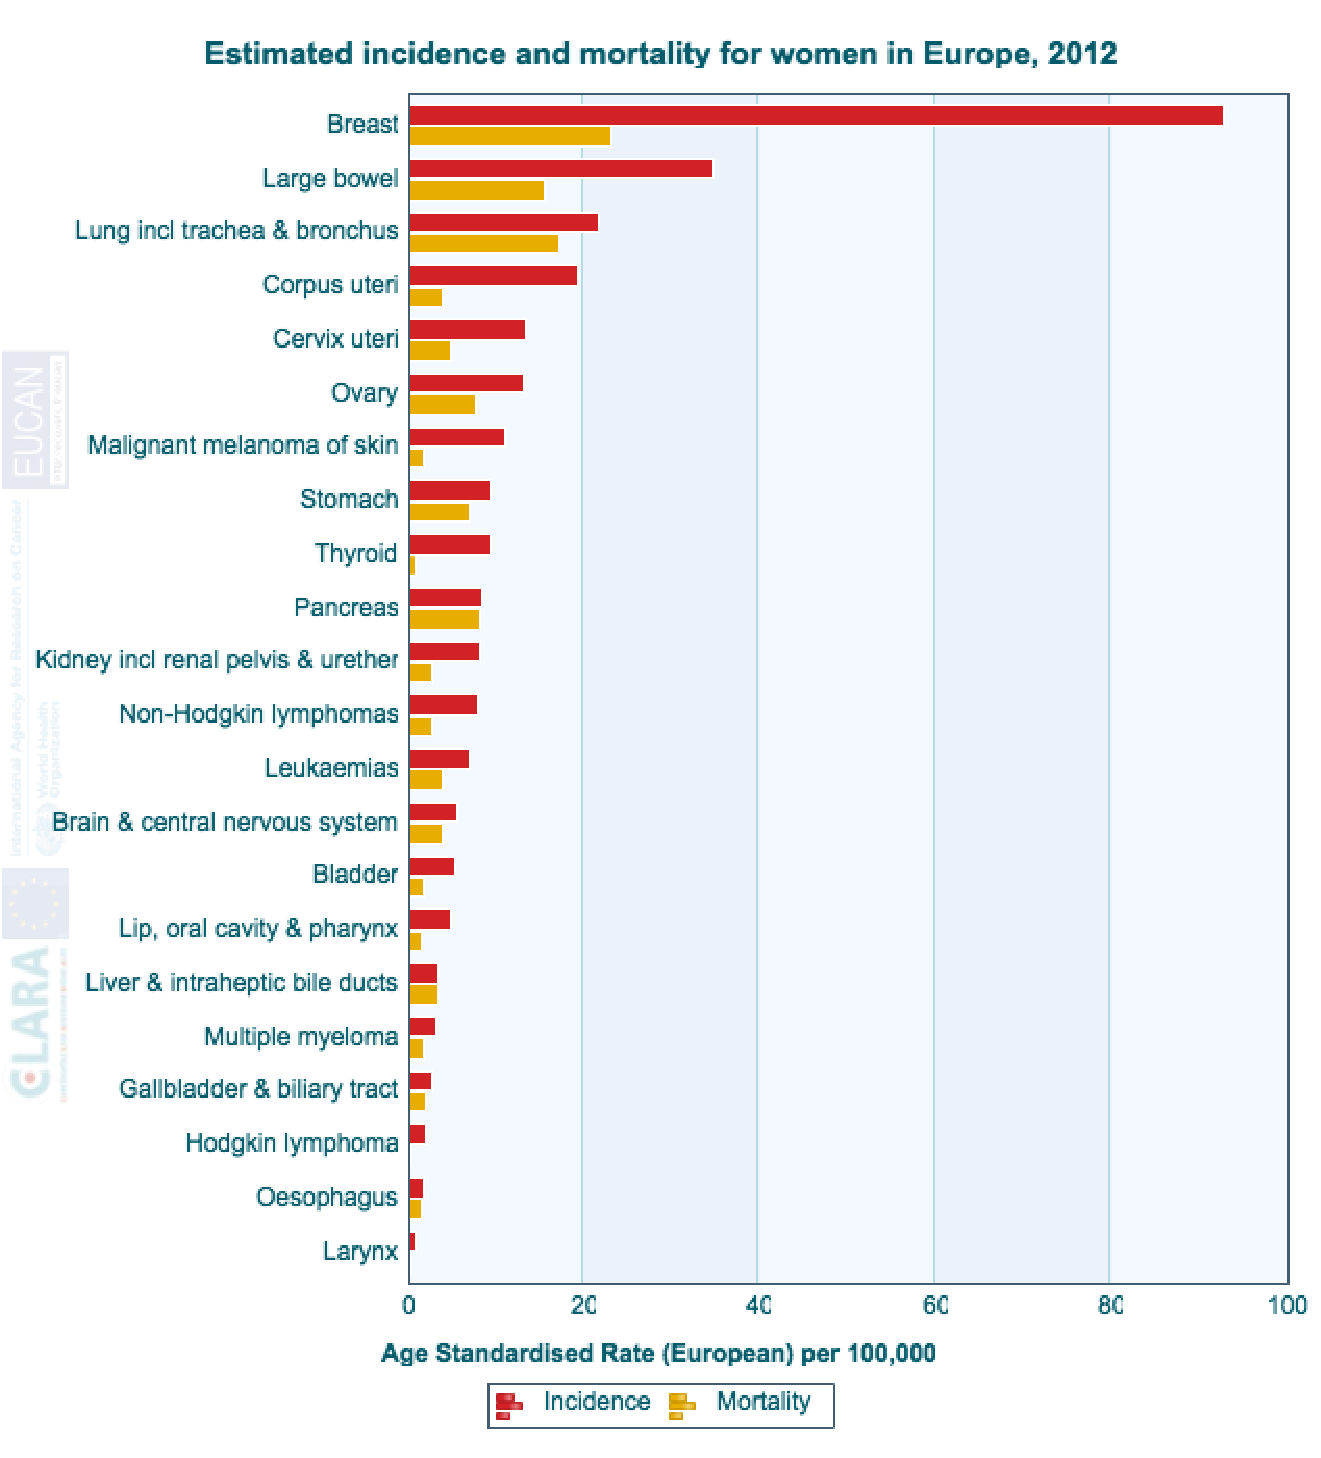
\includegraphics[width=\columnwidth]{slides/IncidenceMortalityBar}
	\>
	\hspace{-0.5cm}
	\<{0.5\linewidth}
		\begin{itemize}
			\item Most common cancer in women
			\item 458,337 new cases in 2012
			\item 131,259 deaths in 2012
		\end{itemize}
		\begin{center}
			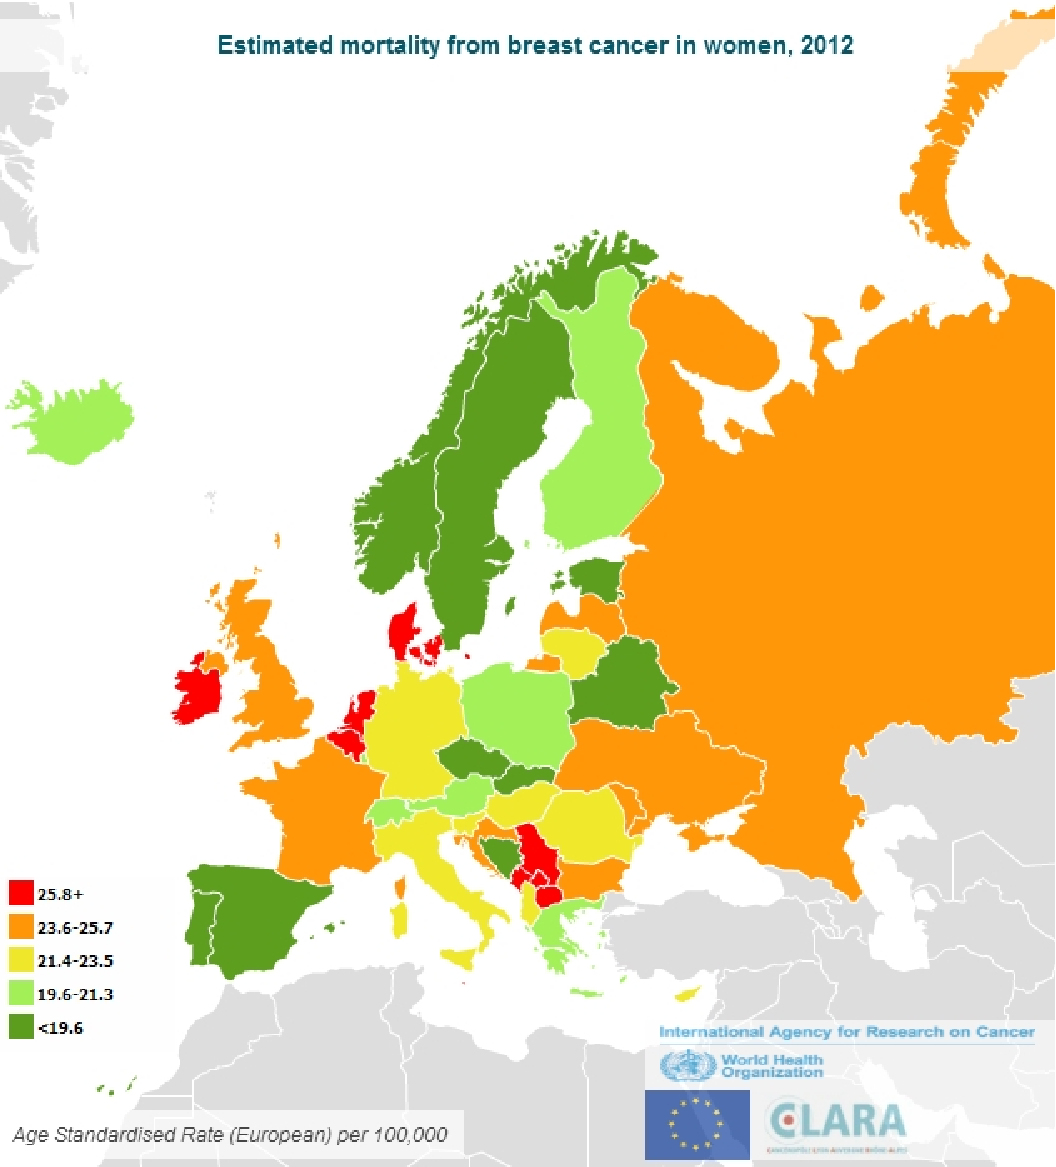
\includegraphics[width=0.85\columnwidth]{slides/MortalityMapSmall}
		\end{center}
	\>
	\)
	
\end{frame}


\subsection{\scshape Cancer prognosis}
\begin{frame}{\insertsubsection}
	
	\begin{itemize}
		\item Prognosis is an estimate of the likely course or outcome
of cancer patients.
	\end{itemize}
	
	\(
	\<{0.4\linewidth}
	\fbox{
		\parbox{0.8\columnwidth}{
		Clinical information
		}
	}
	\begin{equation*}
		\left\{
		\begin{array}{l}
			\textrm{Age at diagnosis} \\
			\textrm{Tumor size} \\
			\textrm{Cancer type/stage} \\
			\textrm{Positive lymph nodes} \\
			\cdots
		\end{array}
		\right.
	\end{equation*}
	
	\only<2->{
	\fbox{
		\parbox{0.9\columnwidth}{
		Molecular information
		}
	}
	\begin{equation*}
		\left\{
		\begin{array}{l}
			\textrm{\alert<3>{Gene expression}} \\
			\textrm{Mutations} \\
			\textrm{Copy number variation} \\
			\cdots
		\end{array}
		\right.
	\end{equation*}
	}
	\>
	
	\<{0.25\linewidth}
	\begin{figure}
	\begin{center}
		\only<1>{
		
\includegraphics[width=0.8\columnwidth]{slides/doctor}
		}
		\only<2->{
		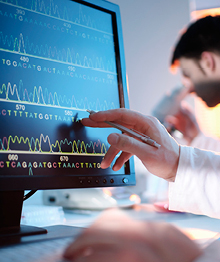
\includegraphics[width=\columnwidth]{slides/Bioinfo}
		}
	\end{center}
	\end{figure}
	\>
	
	\<{0.4\linewidth}
	\only<1>{
		\fbox{
			\parbox{0.7\columnwidth}{
				High/low risk of 5-year relapse
			}
		}
	}
	\only<2->{
		\fbox{
			\parbox{0.92\columnwidth}{
				Prognosis classification
			}
		}
		\fbox{
			\parbox{0.7\columnwidth}{
				Survival analysis
			}
		}
		\fbox{
			\parbox{0.85\columnwidth}{
				Biomarker discovery
			}
		}
	}
	\>
	\)
	
\end{frame}


\subsection{\scshape Gene expression data analysis}
\begin{frame}{\insertsubsection}
	
	\only<1-2>{
	\begin{itemize}
		\item Data: 
		\begin{figure}
			\centering
			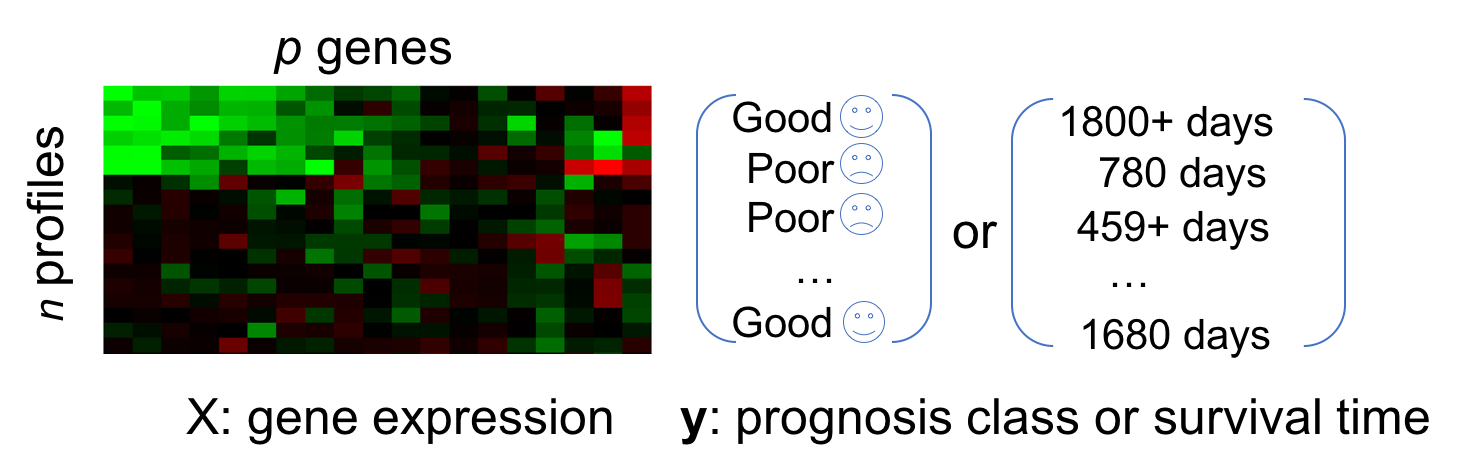
\includegraphics[width=\linewidth]{slides/prognosis}
		\end{figure}
		
		\item Goal: Learn to predict $y$ from a patient's profile $\mathbf{x}$.
		\begin{itemize}
			\item[-] Classification or survival analysis.
			\item[-] Gene selection.
		\end{itemize}
	\end{itemize}
	}
	
	\only<2->{
	\begin{itemize}
		\item \alert<2>{Challenges:}
		\begin{itemize}
			\item[?] High-dimensional ($m \ll n$) noisy data.
			\item[?] Stability and interpretability of gene selection.
		\end{itemize}
	\end{itemize}
	}
	
	\only<3->{
	\begin{itemize}
		\item \alert<3-6>{Initiatives:}
		\begin{itemize}
			\item[$\checkmark$]<3-> Rank-based gene expression analysis.
			\only<3>{
			\begin{figure}
				\centering
				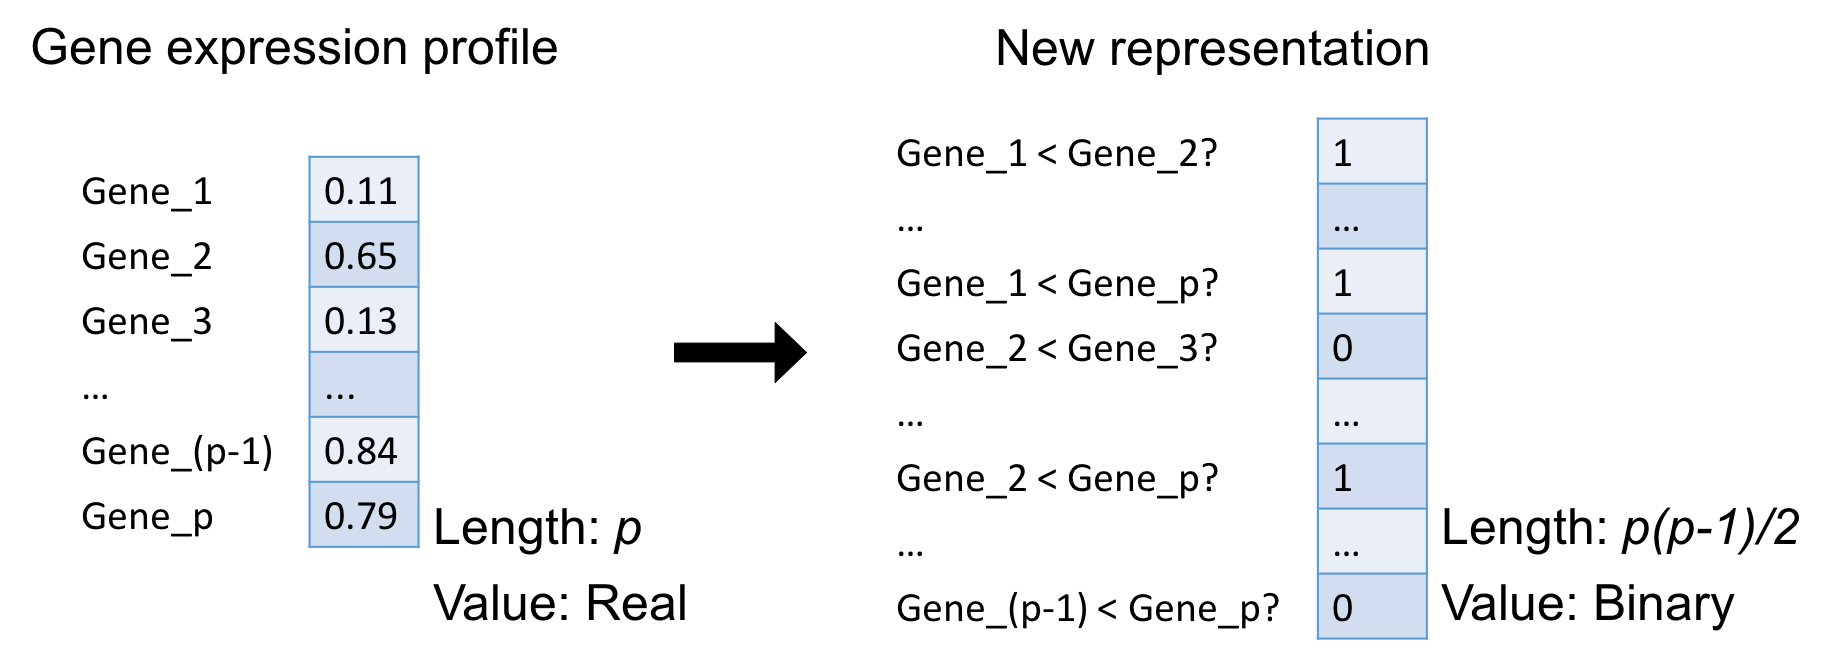
\includegraphics[width=\linewidth]{slides/kendall}
			\end{figure}
			}
			\only<4>{
			\begin{figure}
				\centering
				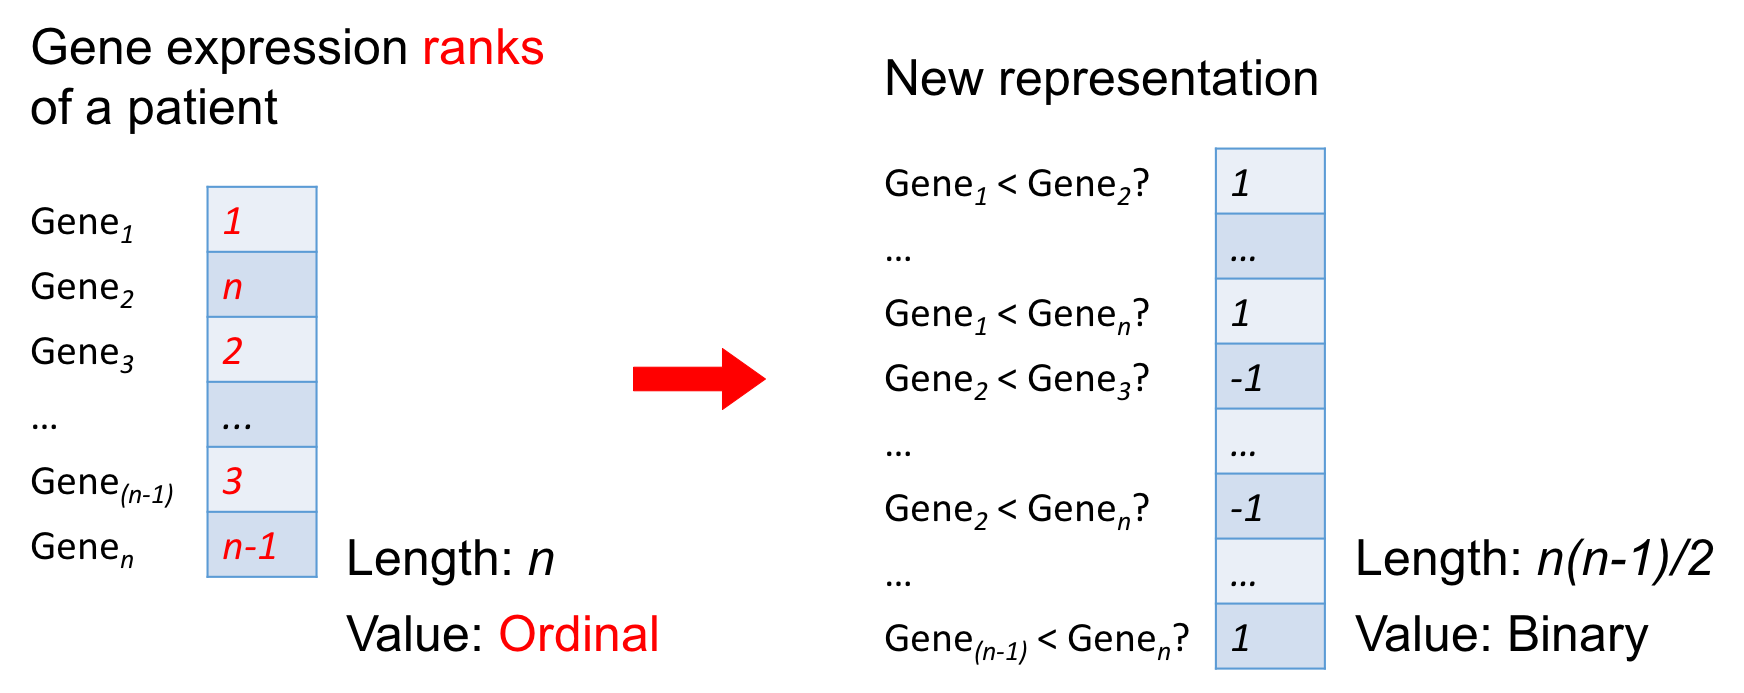
\includegraphics[width=\linewidth]{slides/kendall-2}
			\end{figure}
			}
			
			\item[$\checkmark$]<5-> Network-guided gene/subnetwork selection.
			\only<5>{
			\begin{figure}
				\centering
				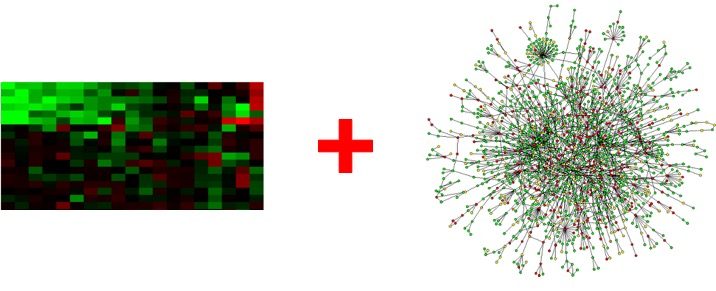
\includegraphics[width=\linewidth]{slides/microarray-ppi}
			\end{figure}
			}
			\only<6>{
			\begin{figure}
				\centering
				\hspace{-2cm}
				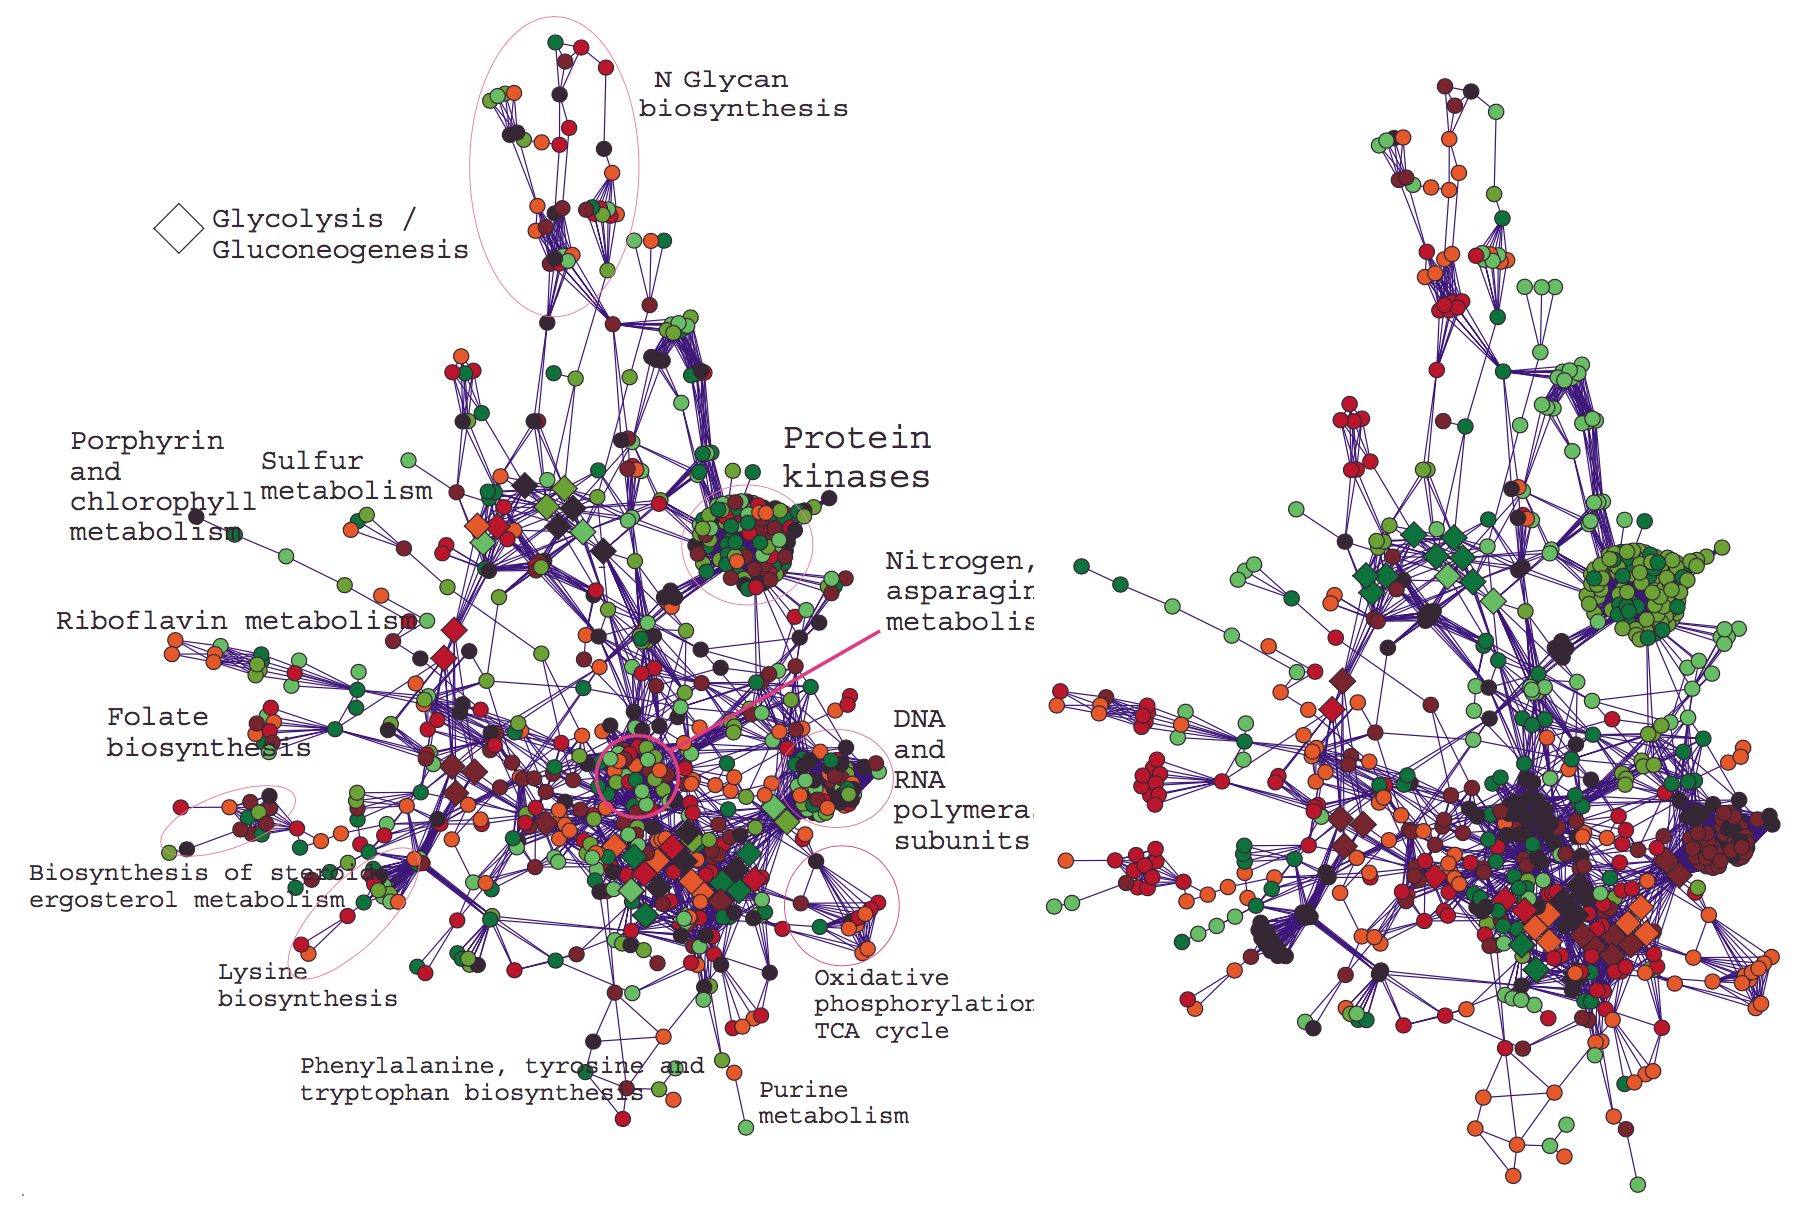
\includegraphics[width=0.75\linewidth]{ch-intro/network}
				\vspace{-0.4cm}
				\caption{Network-free (left) vs network-guided (right) model \cite{Rapaport2007Classification}.}
			\end{figure}
			}
		\end{itemize}
	\end{itemize}
	}
	
	\only<7>{
	\begin{itemize}
		\item \alert<7>{Outline:}
		\begin{itemize}
			\item[\alert<7>{Part 1}] Learning with rank data.
			\item[\alert<7>{Part 2}] Learning on graphs.
		\end{itemize}
	\end{itemize}
	}
	
\end{frame}


\section{\scshape Learning with rank data}


\begin{frame}
	
	\addsectiontitlepage
	
	\(
	\<{0.4\linewidth}
	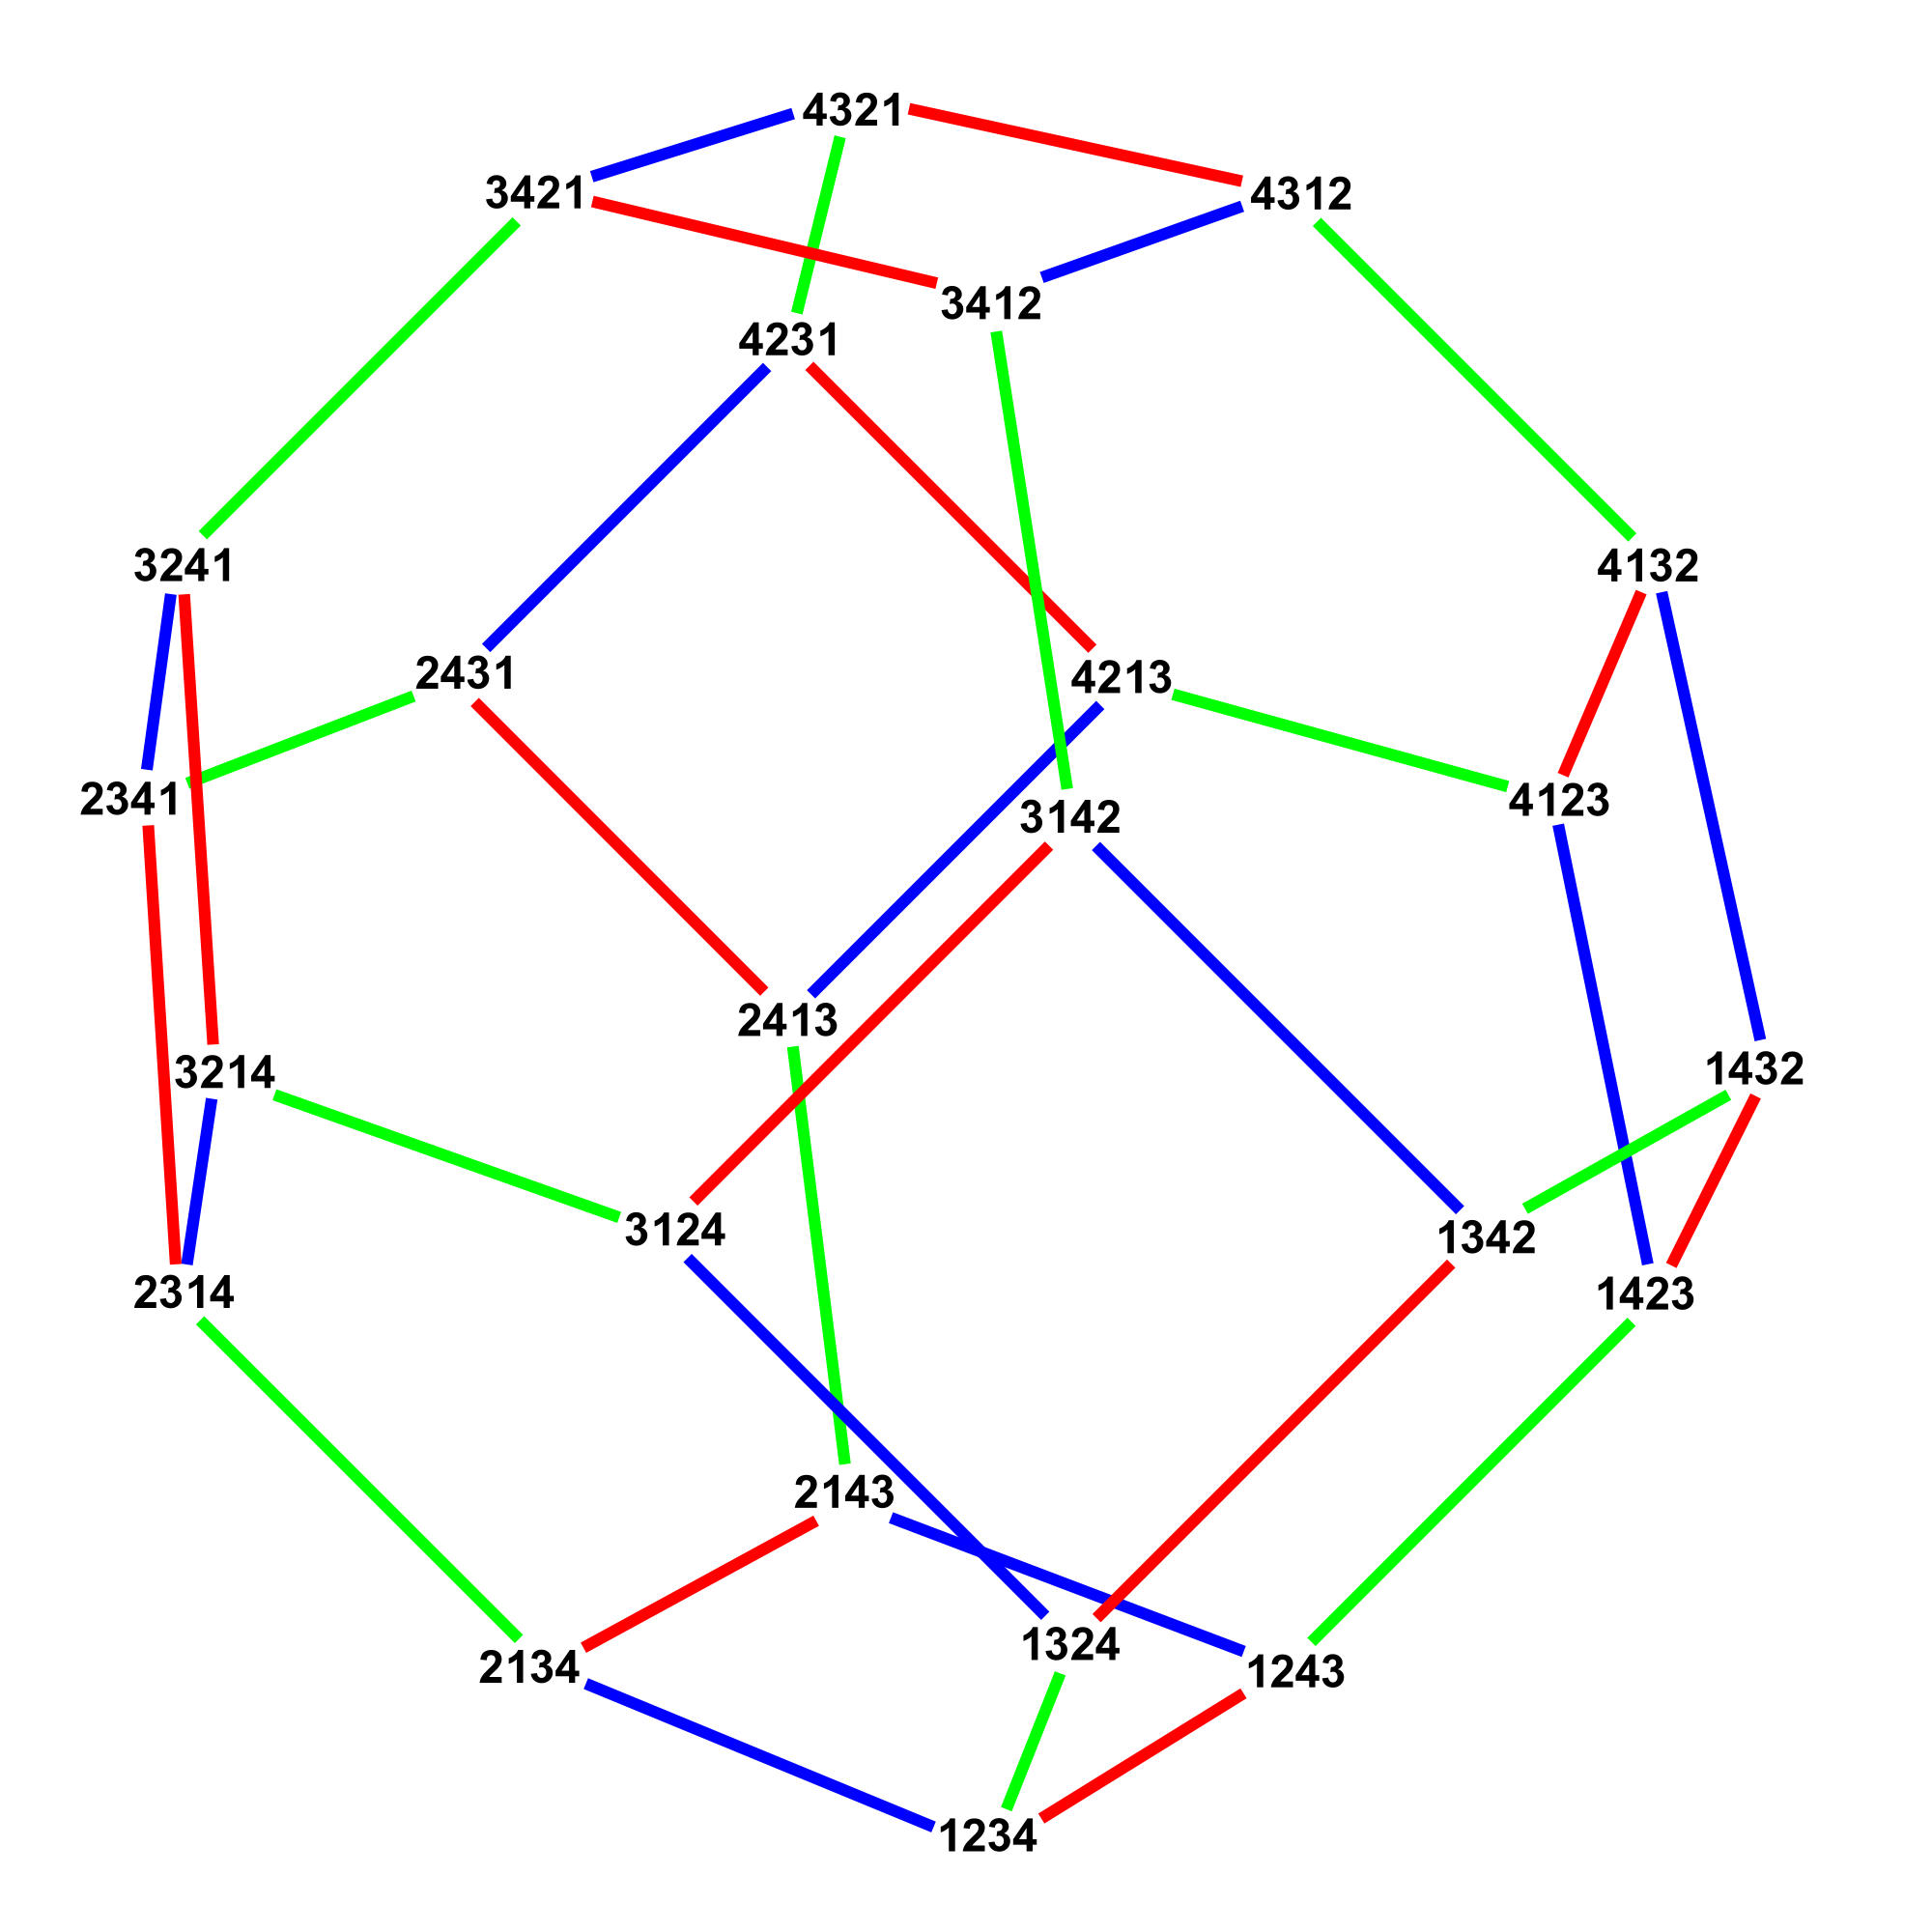
\includegraphics[width=\columnwidth]{ch-kendall/figures/permutahedron}
	\>
	
	\<{0.55\linewidth}
	\begin{footnotesize}
	\textbf{Working Papers and Preprints}
	\begin{itemize}
		\item \nocite{Jiao2017Kendall} Jiao, Y., Vert, J.-P. IEEE TPAMI 2017 (to appear). Preprint HAL-01279273.
	\end{itemize}
	
	\textbf{Published Papers}
	\begin{itemize}
		\item \nocite{Jiao2016Controlling} Jiao, Y., Korba, A., Sibony, E. ICML 2016.
		\item \nocite{Jiao2015Kendall} Jiao, Y., Vert, J.-P. ICML 2015.
	\end{itemize}
	
	\textbf{Software}
	\begin{itemize}
		\item \nocite{Jiao2016kernrank} Jiao, Y. \texttt{kernrank} ver. 1.0.2.
	\end{itemize}
	\end{footnotesize}
	\>
	\)
	
\end{frame}


\subsection{\scshape Motivation recap}
\begin{frame}{\insertsubsection}
	
	\begin{itemize}
		\item Data: 
		\begin{figure}
			\centering
			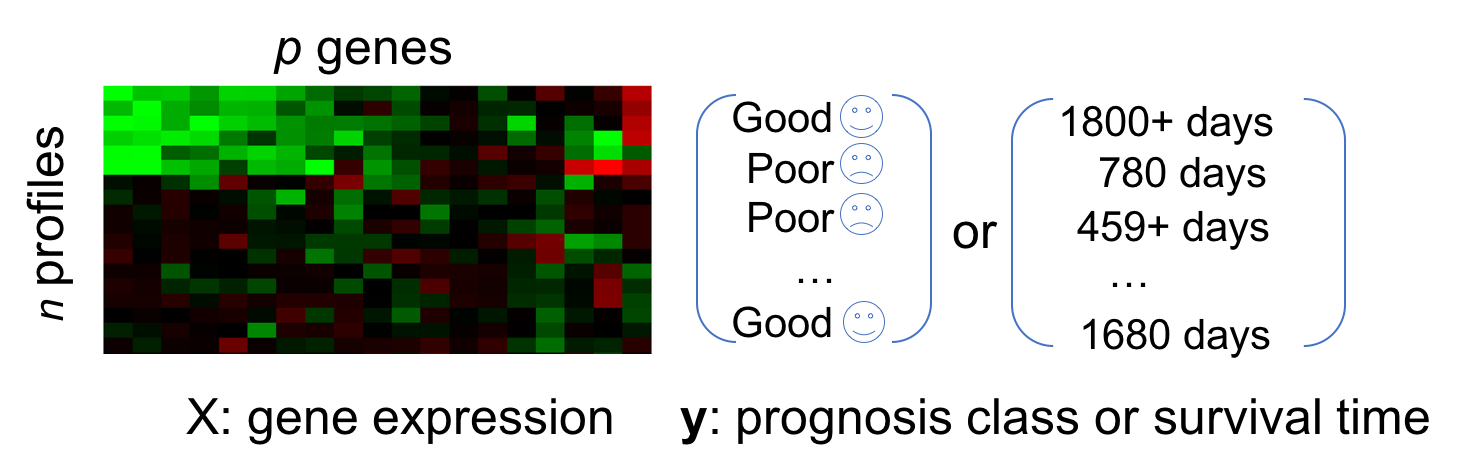
\includegraphics[width=\linewidth]{slides/prognosis}
		\end{figure}
		
		\item Goal: Learn to predict $y$ from a patient's profile $\mathbf{x}$.
		\begin{itemize}
			\item[-] Keep only ordinal ranks but ignore real values.
			\item[-] Classification with kernel machines.
		\end{itemize}
	\end{itemize}
	
\end{frame}


\subsection{\scshape Rank data are everywhere}
\begin{frame}{\insertsubsection}
	
	\([b]
	\<{0.5\linewidth}
		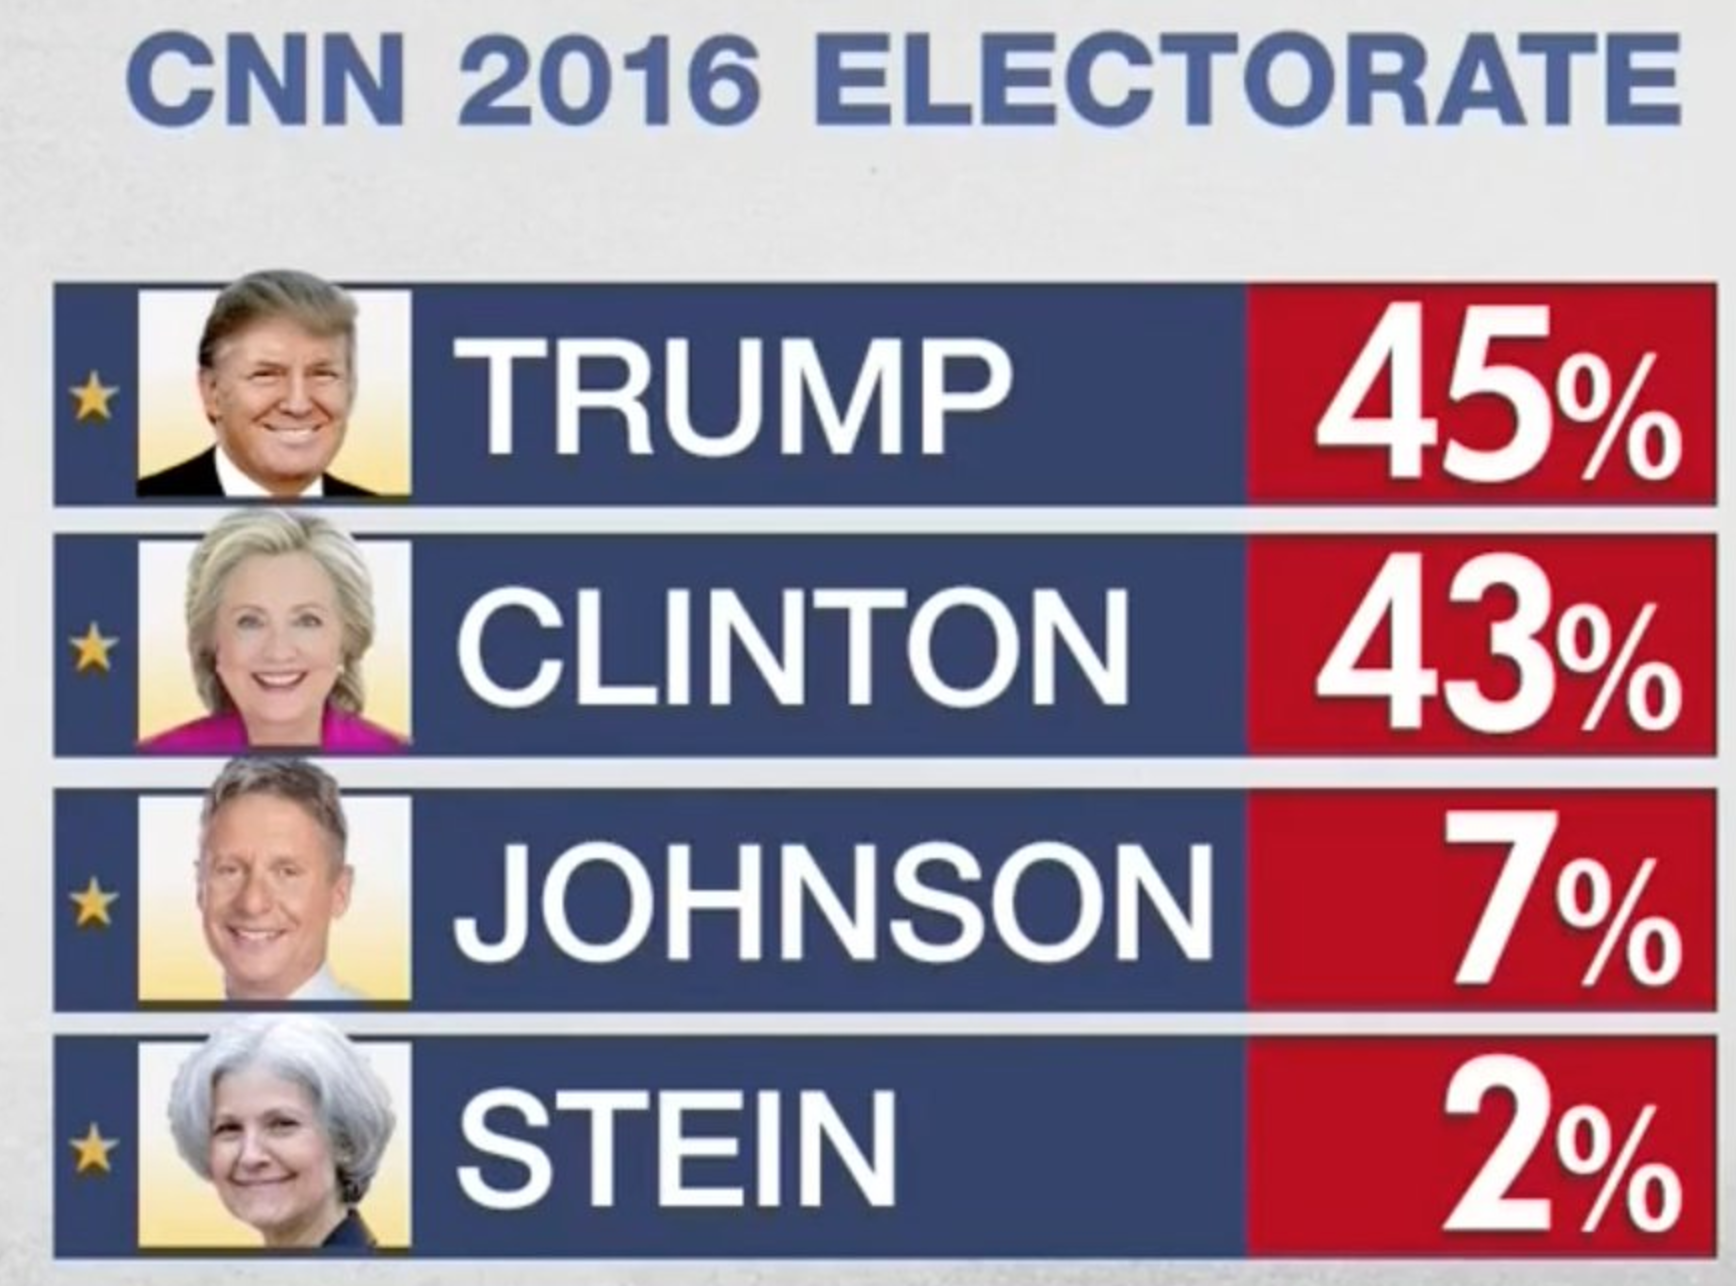
\includegraphics[width=0.9\columnwidth]{slides/USelection}\\
		
\includegraphics[width=\columnwidth]{slides/employee-engagement}
	\>
	\hskip -1cm
	\<{0.6\linewidth}
		\includegraphics[width=0.9\columnwidth]{slides/questionnaire}
	\>
	\)
	
\end{frame}

\subsection{\scshape Total rankings and permutations}
\begin{frame}{\insertsubsection}
	
	\begin{itemize}
		\item<1-> A total ranking $(\xb, \succ)$ is a strict ordering of $n$ items $\{x_1,x_2,\dots,x_n\}\,,$
		$$ x_{i_1} \succ x_{i_2} \succ \cdots \succ x_{i_n}\,. $$
		\item<1-> A permutation $\sigma \in \Sn$ is a rearrangement of $n$ indices,
		$$ \sigma: \{1,2,\dots,n\} \to \{1,2,\dots,n\} \mbox{ such that } \sigma(i)\neq \sigma(j) \mbox{ for } i\neq j\,.$$
		\item<2-> A total ranking is \alert<2>{equivalently represented} by a permutation if $\sigma$ maps item index to item rank, e.g.,
		\begin{equation*}
		\begin{split}
			& x_2 \succ x_4 \succ x_3 \succ x_1 \\
			\Longleftrightarrow \sigma = & 
				\left(\begin{array}{llll}
					1 & 2 & 3 & 4 \\
					1 & 4 & 2 & 3 \\
				\end{array}\right)
				\left.\begin{array}{l}
					\mbox{--- index} \\
					\mbox{--- rank} \\
				\end{array}\right. \\
				(\mbox{or written } & \sigma = (1 , 4 , 2 , 3) \mbox{ for simplicity}) \\
			\Longleftrightarrow \sigma(1)=1 &, \sigma(2)=4, \sigma(3)=2, \sigma(4)=3\,.
		\end{split}
		\end{equation*}
	\end{itemize}
	
\end{frame}

\subsection{\scshape Kendall kernel for permutations}
\begin{frame}{\insertsubsection}
	
	\only<1-3>{
	\([c]
	\<{0.7\linewidth}
		\begin{itemize}
			\item<1-> Kendall tau distance \cite{Kendall1938New} counts the number of discordant pairs between permutations, i.e., 
			\begin{equation*}
			\begin{split}
				d (\sigma, & \sigma') := \# \big\{ (i,j) | \mbox{ for } i < j \,, \\
				& (\sigma(i)-\sigma(j))(\sigma'(i)-\sigma'(j)) < 0 \big\} \,.
			\end{split}
			\end{equation*}
			
			\item<2-> Kendall tau correlation \cite{Kendall1938New} for permutations is defined as
			$$ K_\tau(\sigma, \sigma') := 1 - \frac{2d(\sigma, \sigma')}{{n\choose 2}} \,. $$
		\end{itemize}
	\>
	
	\vrule{}
	
	\<{0.4\linewidth}
		\vskip 0.1cm
		E.g.,
		\vskip 0.2cm
		\begin{tabular}{c|ccccc}\hline
			index $e$ & 1 & 2 & 3 & 4 \\ \hline
			rank $\sigma$ & 2 & 3 & 4 & 1 \\
			rank $\sigma'$ & 3 & 1 & 4 & 2 \\\hline
		\end{tabular}
		
		\vskip 0.2cm
		$$ d(\sigma,\sigma') = 2 $$
		
		\vskip 1cm
		\uncover<2>{
		$$ K_\tau(\sigma,\sigma') = \frac{1}{3} $$
		}
	\>
	\)
	}
	
	\only<3->{
	\begin{thm}[Main theorem \cite{Jiao2015Kendall}]
		$K_\tau$ is a positive definite kernel on $\Sn$, and $d$ is a negative definite kernel on $\Sn$.
	\end{thm}
	}
	
	\only<4>{
	Recall from introduction:
	\begin{figure}
		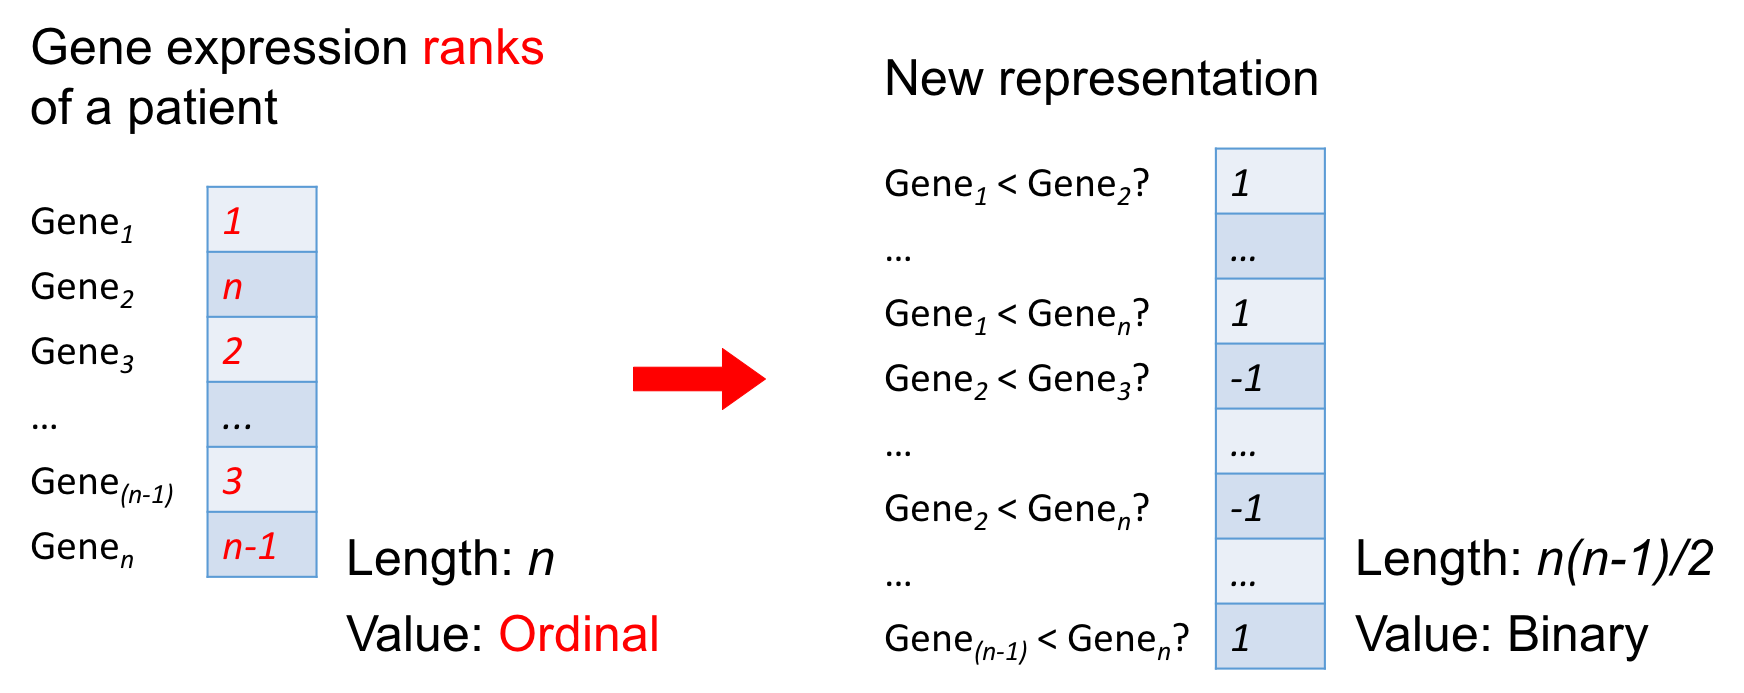
\includegraphics[width=\linewidth]{slides/kendall-2}
	\end{figure}
	}
	
	\only<5->{
	\begin{proof}
	\footnotesize
		Consider explicitly the \alert<5>{Kendall embedding} defined as
		$$ \phi:\Sn \rightarrow \RR^{{n \choose 2}}, \sigma \mapsto \left( \sgn(\sigma(i)-\sigma(j)) \right)_{1\leq i < j \leq n} \,. $$
		Up to constant scaling, we have
		\begin{eqnarray*}
			\alert<5>{\mbox{Kendall kernel:}} \quad K_\tau(\sigma, \sigma') & = & \phi(\sigma)^\top \phi(\sigma') \,, \\
			\alert<5>{\mbox{Kendall distance:}} \quad d(\sigma, \sigma') & = & \nm{\phi(\sigma) - \phi(\sigma')}^2 \,.
		\end{eqnarray*}
	\end{proof}
	}
	
	\only<6>{
	\begin{thm}[Kernel trick \cite{Knight1966Computer}]
		Both quantities $K_\tau$ and $d$ can be evaluated in \alert<6>{$O(n\log n)$} time.
	\end{thm}
	}
	
\end{frame}


\subsection{\scshape Application (1/3): Biomedical classification}
\begin{frame}{\insertsubsection}
	
	\only<1>{
	\begin{itemize}
		\item Datasets:
	\end{itemize}
		\vskip -0.4cm
		\begin{table}
		\scriptsize
			\begin{tabular}{cccc}
			\hline
			Dataset & No. of features & \multicolumn{2}{c}{No. of samples in each class (training/test)} \\
			& & $C_1$ & $C_2$ \\
			\hline
			Breast Cancer 1 & 23624 & 44/7 (Non-relapse) & 32/12 (Relapse) \\
			Breast Cancer 2 & 22283 & 142 (Non-relapse) & 56 (Relapse) \\
			Breast Cancer 3 & 22283 & 71 (Poor Prognosis) & 138 (Good Prognosis) \\
			Colon Tumor & 2000 & 40 (Tumor) & 22 (Normal) \\
			Lung Cancer 1 & 7129 & 24 (Poor Prognosis) & 62 (Good Prognosis) \\
			Lung Cancer 2 & 12533 & 16/134 (ADCA) & 16/15 (MPM) \\
			Medulloblastoma & 7129 & 39 (Failure) & 21 (Survivor) \\
			Ovarian Cancer & 15154 & 162 (Cancer) & 91 (Normal) \\
			Prostate Cancer 1 & 12600 & 50/9 (Normal) & 52/25 (Tumor) \\
			Prostate Cancer 2 & 12600 & 13 (Non-relapse) & 8 (Relapse) \\
			\hline
			\end{tabular}
		\end{table}
		\vskip -0.1cm
		
	\begin{itemize}
		\item Methods:
		\begin{itemize}
			\item[-] Kernel machines: \alert{Support Vector Machines (SVM)} and Kernel Fisher Discriminant (KFD) \alert{with Kendall kernel}, linear kernel, Gaussian RBF kernel, polynomial kernel.
			\item[-] Baseline classifiers: Top Scoring Pairs (TSP) \cite{Tan2005Simple}.
			\item[-] Hybrid schemes: SVM + TSP feature selection algorithm.
		\end{itemize}
	\end{itemize}
	}
	
	\only<2->{
	\([c]
	\<{0.65\linewidth}
		\begin{figure}
			\only<2>{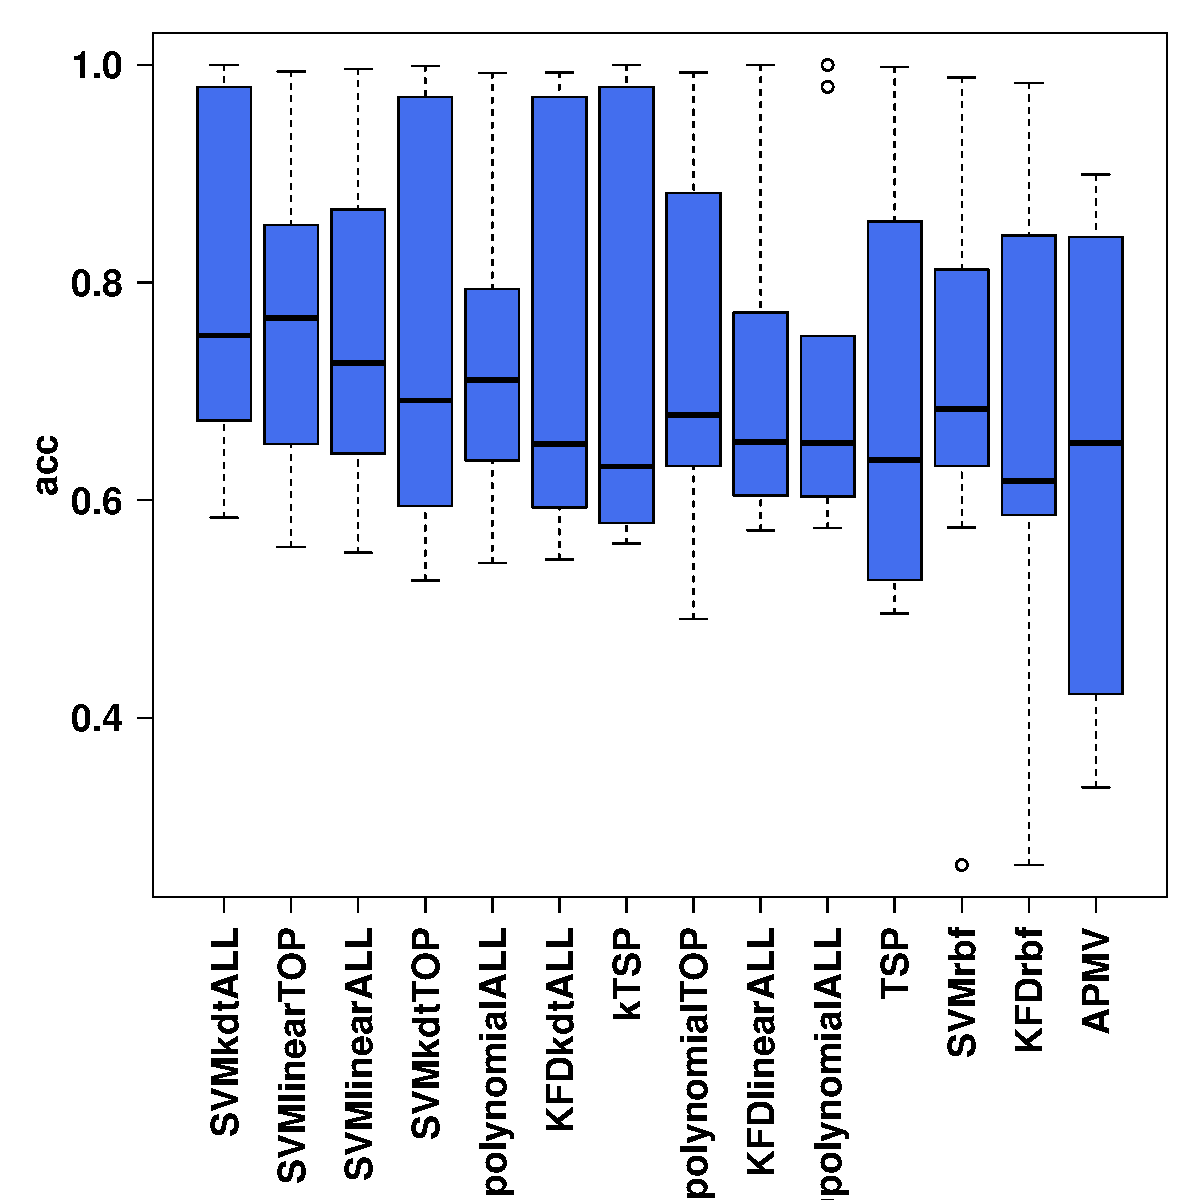
\includegraphics[width=\columnwidth]{ch-kendall/clasf_results/acc_plot}}
			\only<3>{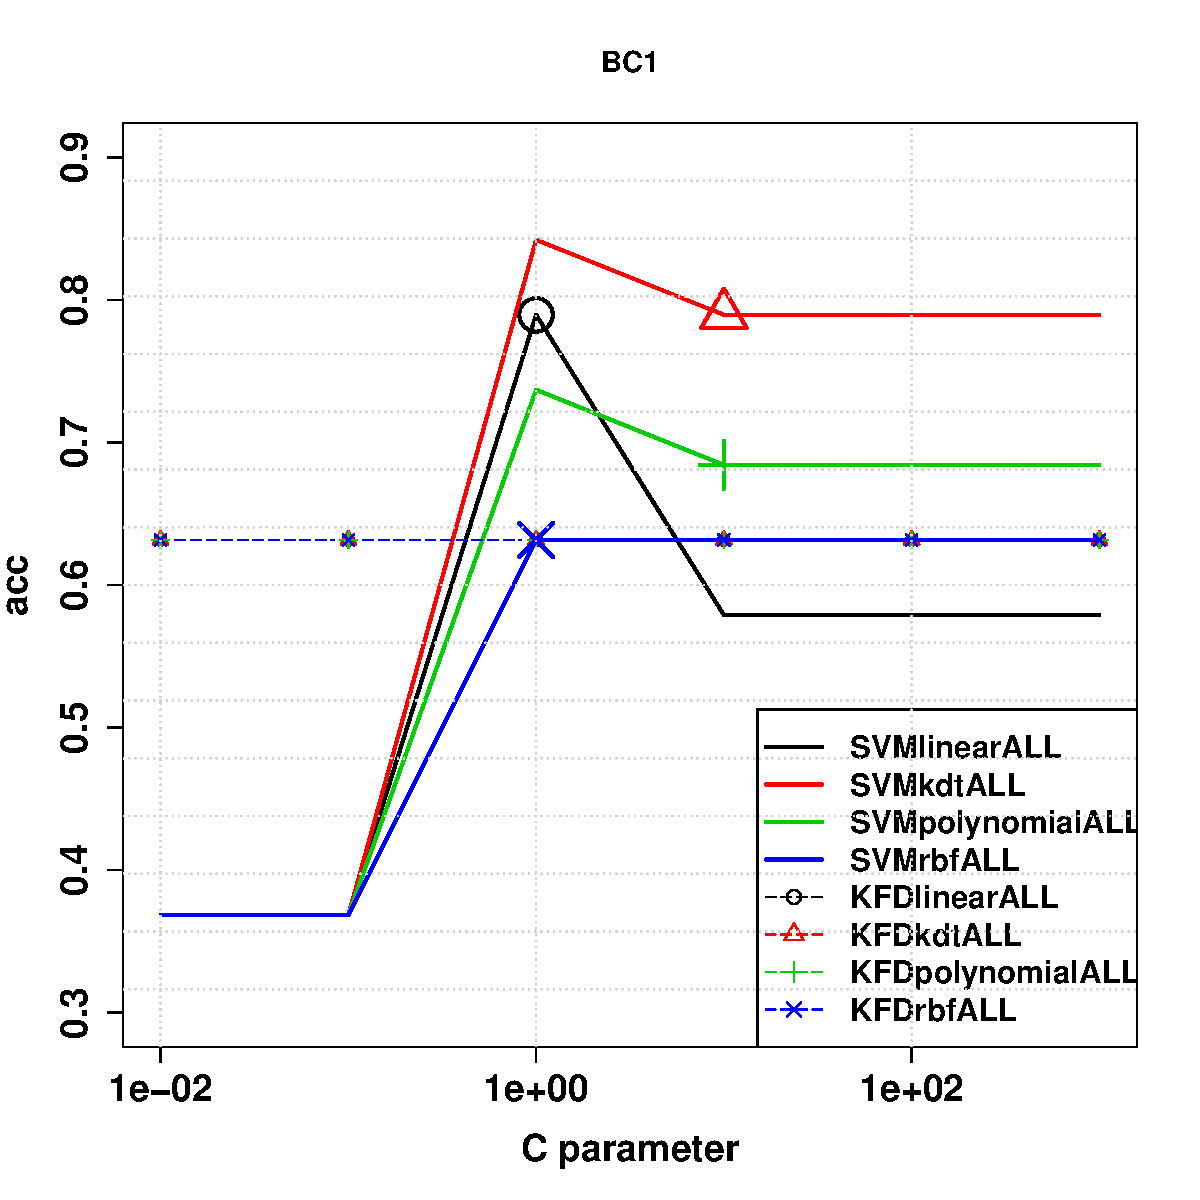
\includegraphics[width=\columnwidth]{ch-kendall/clasf_results/acc_perfSVM}}
			\only<4>{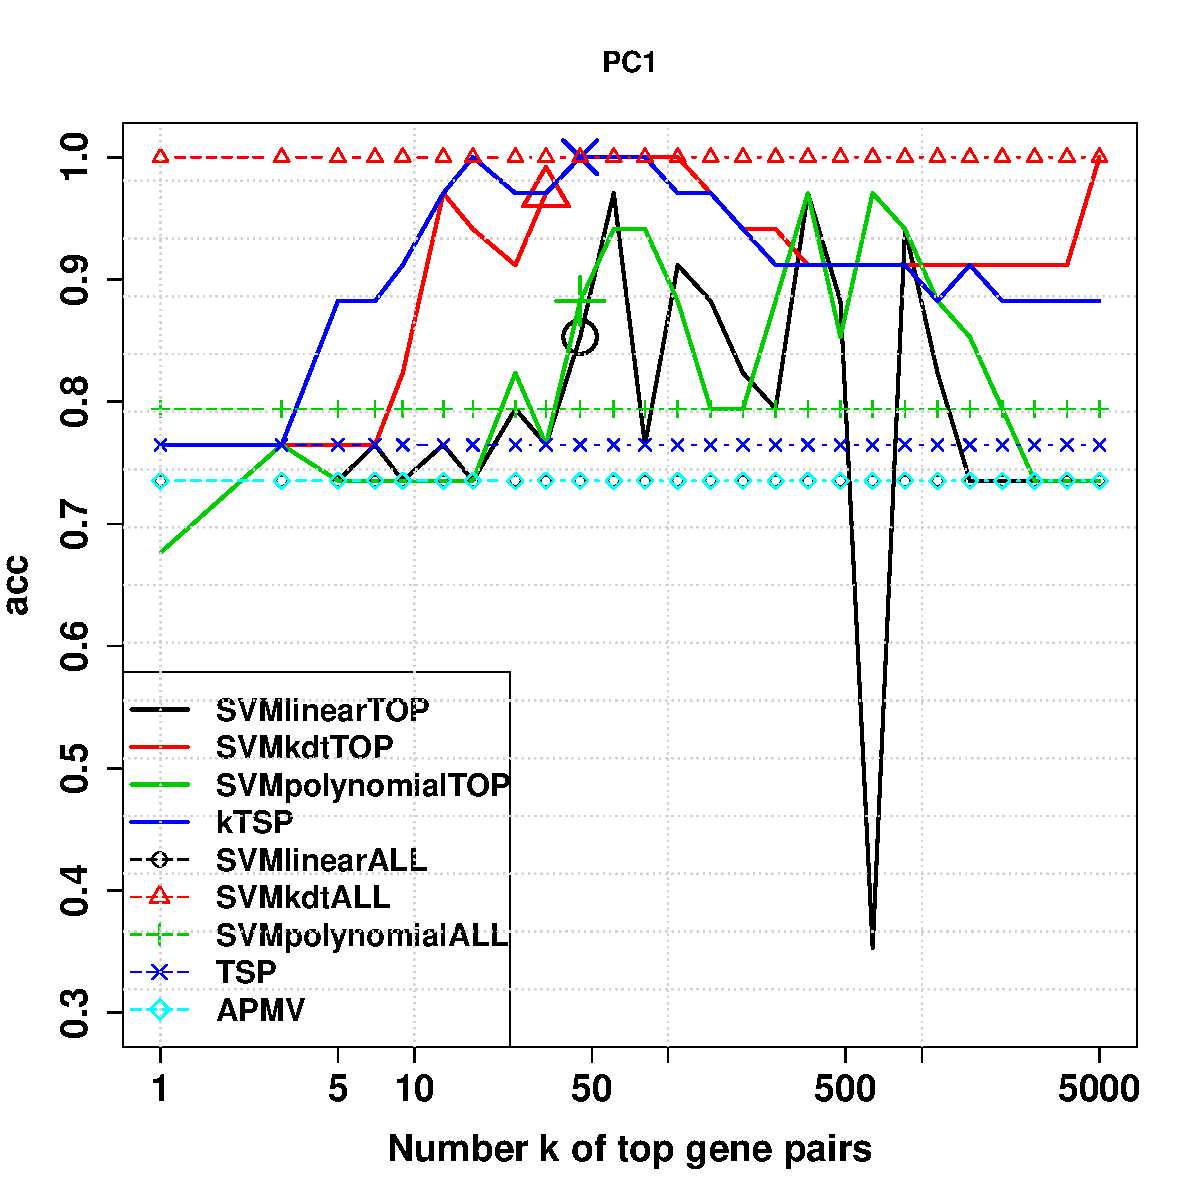
\includegraphics[width=\columnwidth]{ch-kendall/clasf_results/acc_perfFS}}
		\end{figure} 
	\>
	\hspace{-0.3cm}
	\<{0.5\linewidth}
		Kendall kernel SVM has
		\begin{itemize}
			\item<2-4> \alert<2>{Competitive accuracy!}
			\item<3-4> \alert<3>{Less sensitivity to regularization parameter!}
			\item<4> \alert<4>{No need for feature selection!}
		\end{itemize}
	\>
	\)
	}
	
\end{frame}


\subsection{\scshape Application (2/3): Rank aggregation}
\begin{frame}{\insertsubsection}
	
	\only<1>{
	\begin{itemize}
		\item Rank aggregation: \alert<1>{Given a collection} of permutations $\{\sigma_i\}_{i=1}^m \in \Sn^m$, \alert<1>{find a consensus permutation} $\sigstar \in \Sn$ that ``best'' summarizes them.
	\end{itemize}
	\begin{figure}
		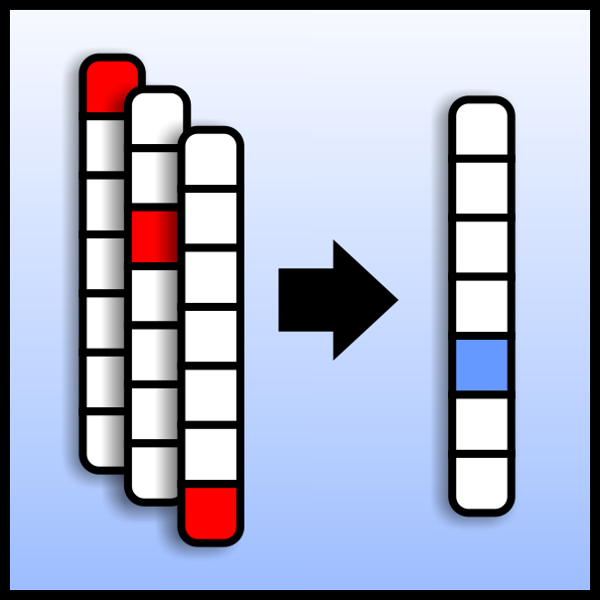
\includegraphics[width=0.5\linewidth]{slides/rankaggregation}
	\end{figure}
	}
	
	\only<2-7>{
	\begin{itemize}
		\item	Kemeny aggregation: Given $\DD := \{\sigma_i\}_{i=1}^m \in \Sn^m$,
		\only<2-5>{
			\only<2-3>{
			\begin{equation*}
			\sigstar \in \argmin_{\sigma \in \Sn} \sum_{i=1}^{m} d(\sigma,\sigma_i) \,.
			\end{equation*}
			}
			\only<4->{
			\begin{equation*}
			\begin{split}
			\sigstar & \in \argmin_{\sigma \in \Sn} \sum_{i=1}^{m} \alert<4>{ \nm{\phi(\sigma) - \phi(\sigma_i)}^2 }
			\only<5>{ \\
				& = \argmin_{\sigma \in \Sn} \nm{ \phi(\sigma) - \frac{1}{m} \sum_{i=1}^m \phi(\sigma_i) }^2
			}
			\,.
			\end{split}
			\end{equation*}
			}
		}
		\only<6->{
		\([c]
		\<{0.6\columnwidth}
			\begin{itemize}
				\item[\alert<6>{Step 1}] Compute the mean embedding of $\DD$ in \alert<6>{$O(mn^2)$} time by
				$$ \phi(\DD) := \frac{1}{m} \sum_{i=1}^m \phi(\sigma_i) \,. $$
				\item[\alert<6>{Step 2}] Find a Kemeny consensus $\sigstar$ by solving the \alert<6>{NP-hard} problem:
				$$ \sigstar \in \argmin_{\sigma \in \Sn} \nm{ \phi(\sigma) - \phi(\DD) }^2 \,. $$
			\end{itemize}
		\>
		\hspace{-0.5cm}
		\<{0.45\linewidth}
			\begin{figure}
				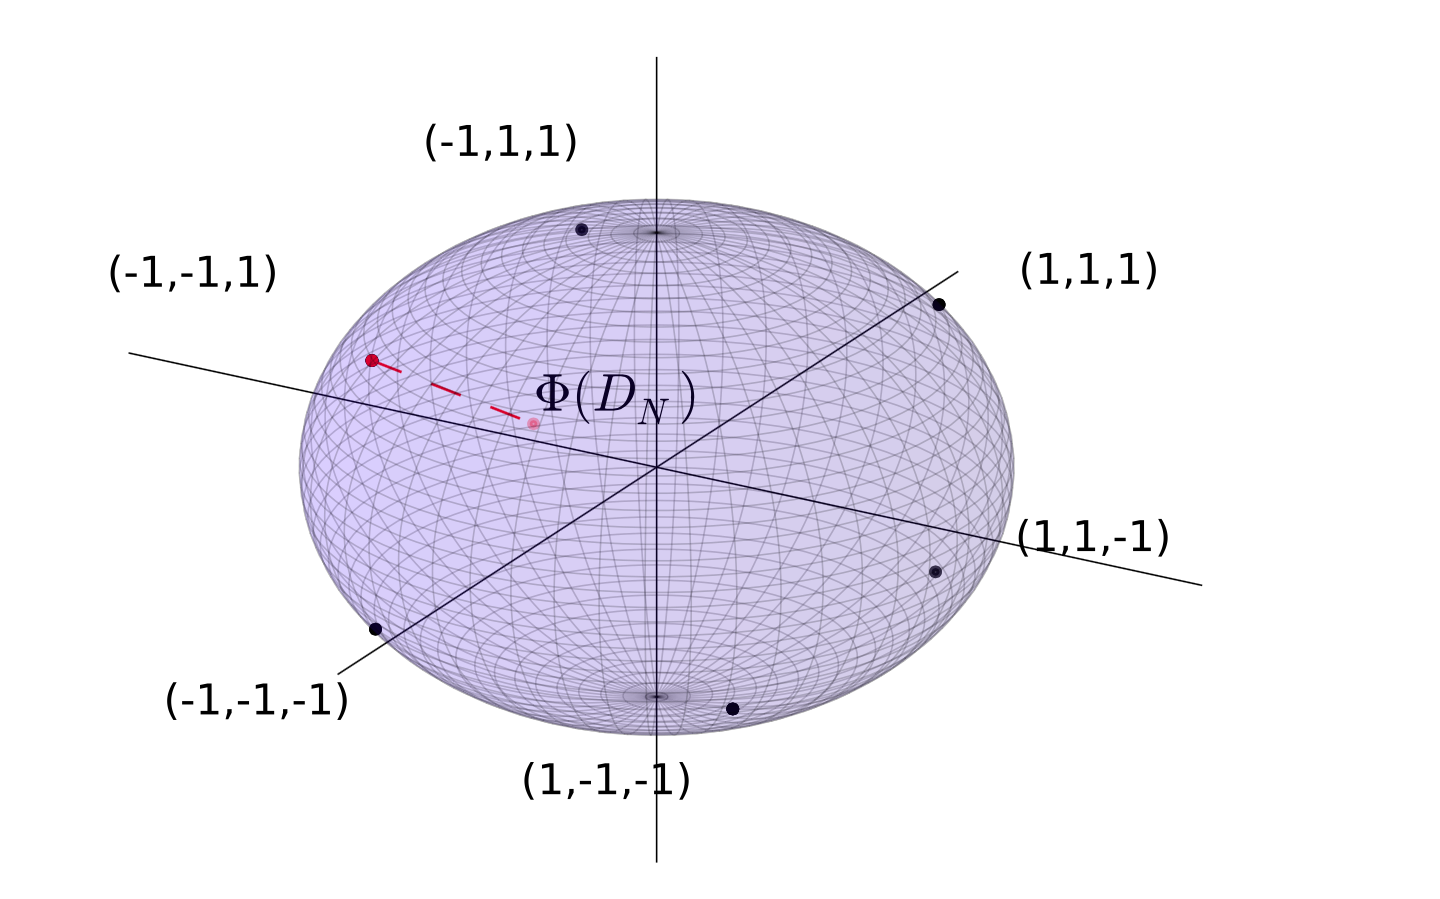
\includegraphics[trim=2cm 2.5cm 3.5cm 3cm, clip=true, width=\textwidth, height=1.3in]{ch-kemeny/figures/3d1test}
				\caption{Kemeny aggregation for $n=3$.}
			\end{figure}
		\>
		\)
		}
	\end{itemize}
	}
		
	\only<3-7>{
	\begin{itemize}
		\item \alert<3>{Dilemma:} Kemeny consensus $\sigstar$ is desirable but NP-hard to find\only<7->{, and usually \alert<7->{approximated by $\sigma$} from a tractable procedure in practice}.
	\end{itemize}
	}
	
	\only<8->{
	\begin{thm}[Tractable approx bound \cite{Jiao2016Controlling}]
		If the Euclidean angle $\theta(\sigma)$ between $\phi(\sigma)$ and $\phi(\DD)$ is less than $\frac{\pi}{2}$, then
		$$d(\sigma, \sigstar) \leq \left\lfloor {n \choose 2} \sin^2(\theta(\sigma)) \right\rfloor \,,$$
		where $\lfloor \cdot \rfloor$ denotes the integer part of a real number.
	\end{thm}
	}
	
\end{frame}


\subsection{\scshape Application (3/3): Cluster analysis}
\begin{frame}{\insertsubsection}
	
	\only<1>{
	\begin{itemize}
		\item Cluster analysis: \alert<1>{Given a collection} of permutations $\{\sigma_i\}_{i=1}^m \in \Sn^m$, \alert<1>{assign each permutation} into one of $c$ clusters $\{S_j\}_{j=1}^c$.
	\end{itemize}
	\begin{figure}
		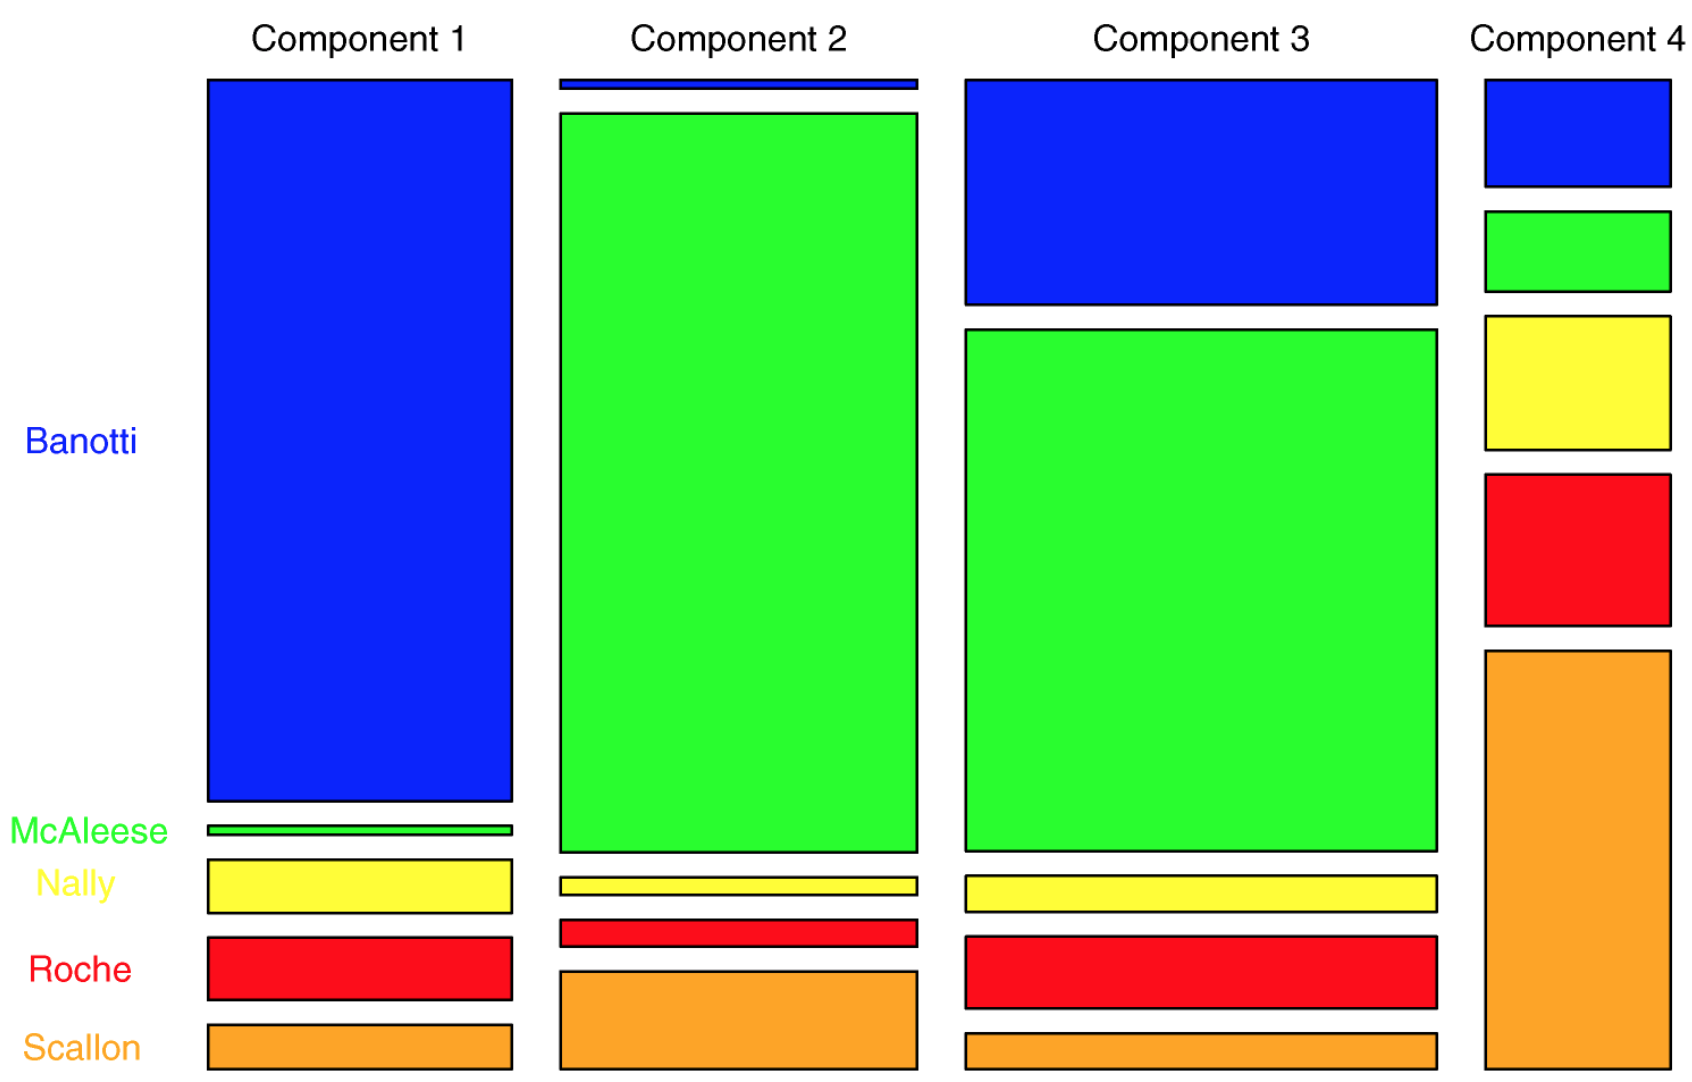
\includegraphics[width=0.7\linewidth]{slides/clusterRank}
		\caption{An example of voting blocs in Irish electorate \cite{Gormley2008Exploring}.}
	\end{figure}
	}
	
	\only<2-3>{
	\begin{itemize}
		\item Cluster analysis with \alert{\only<3->{kernel} $k$-means}: Given a collection of permutations $\{\sigma_i\}_{i=1}^m \in \Sn^m$, assign each permutation into one of $c$ clusters $\{S_j\}_{j=1}^c$ by solving
		\only<2>{
			$$
			\argmin_{\left\{S_j, \pi_j \in \Sn\right\}_{j=1}^c} \sum_{j=1}^{c} \sum_{i: \sigma_i \in S_j} d(\pi_j, \sigma_i) \,,
			$$
			where each $\pi_j$ is the \alert{center permutation} of cluster $S_j$.}
		\only<3->{
			$$
			\argmin_{\left\{S_j, \mu_j \in \RR^{{n \choose 2}}\right\}_{j=1}^c} \sum_{j=1}^{c} \sum_{i: \sigma_i \in S_j} \nm{\mu_j - \phi(\sigma_i)}^2 \,,
			$$
			where each $\mu_j$ is the \alert{center embedding} of cluster $S_j$.
		}
		
		\item Lloyd's algorithm applies\only<3->{ with \alert{kernel trick}}:
		\begin{figure}
		\only<2>{
			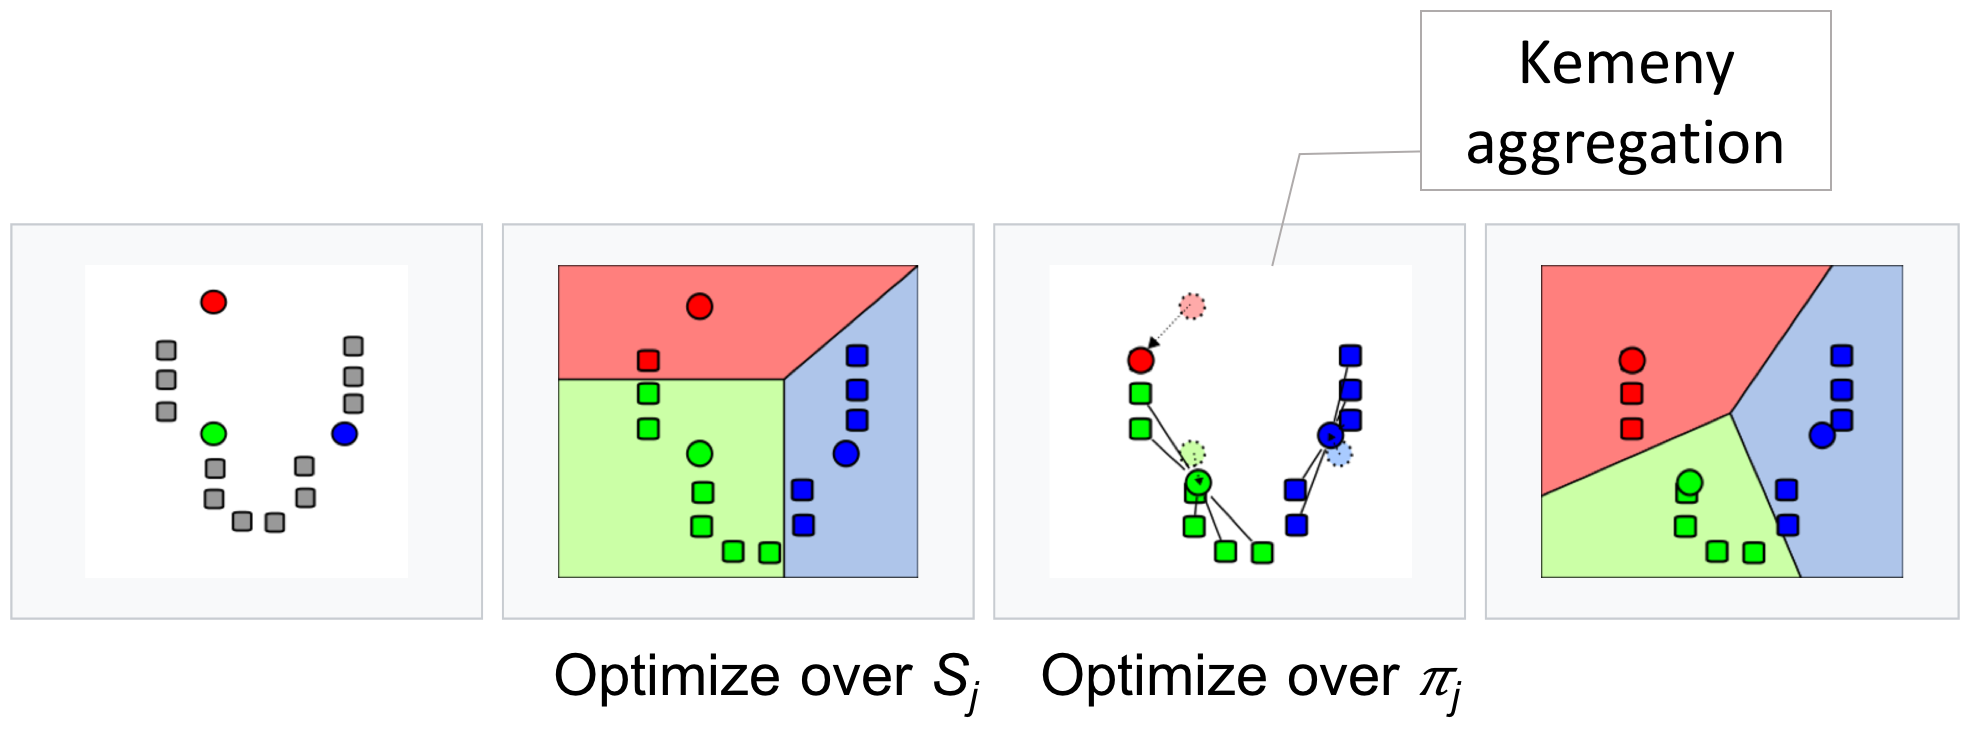
\includegraphics[width=0.9\linewidth]{slides/kmeans}
		}
		\only<3->{
			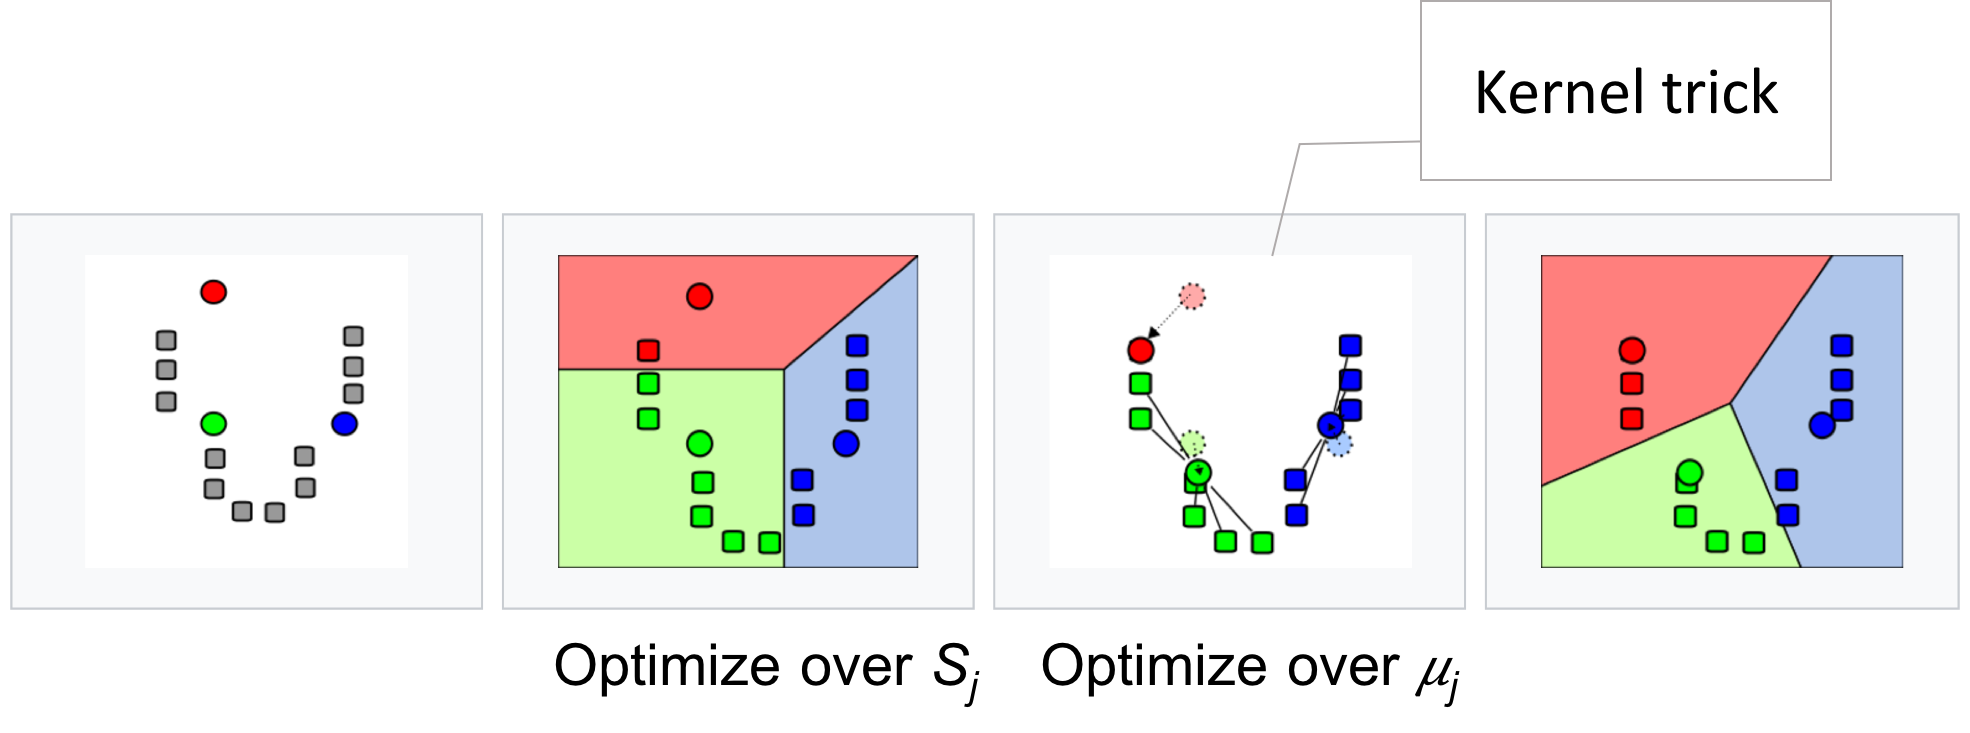
\includegraphics[width=0.9\linewidth]{slides/kkmeans}
		}
		\end{figure}
	\end{itemize}
	}
	
%	\only<4->{
%	\([c]
%	\<{0.65\linewidth}
%		\begin{figure}
%			\only<4>{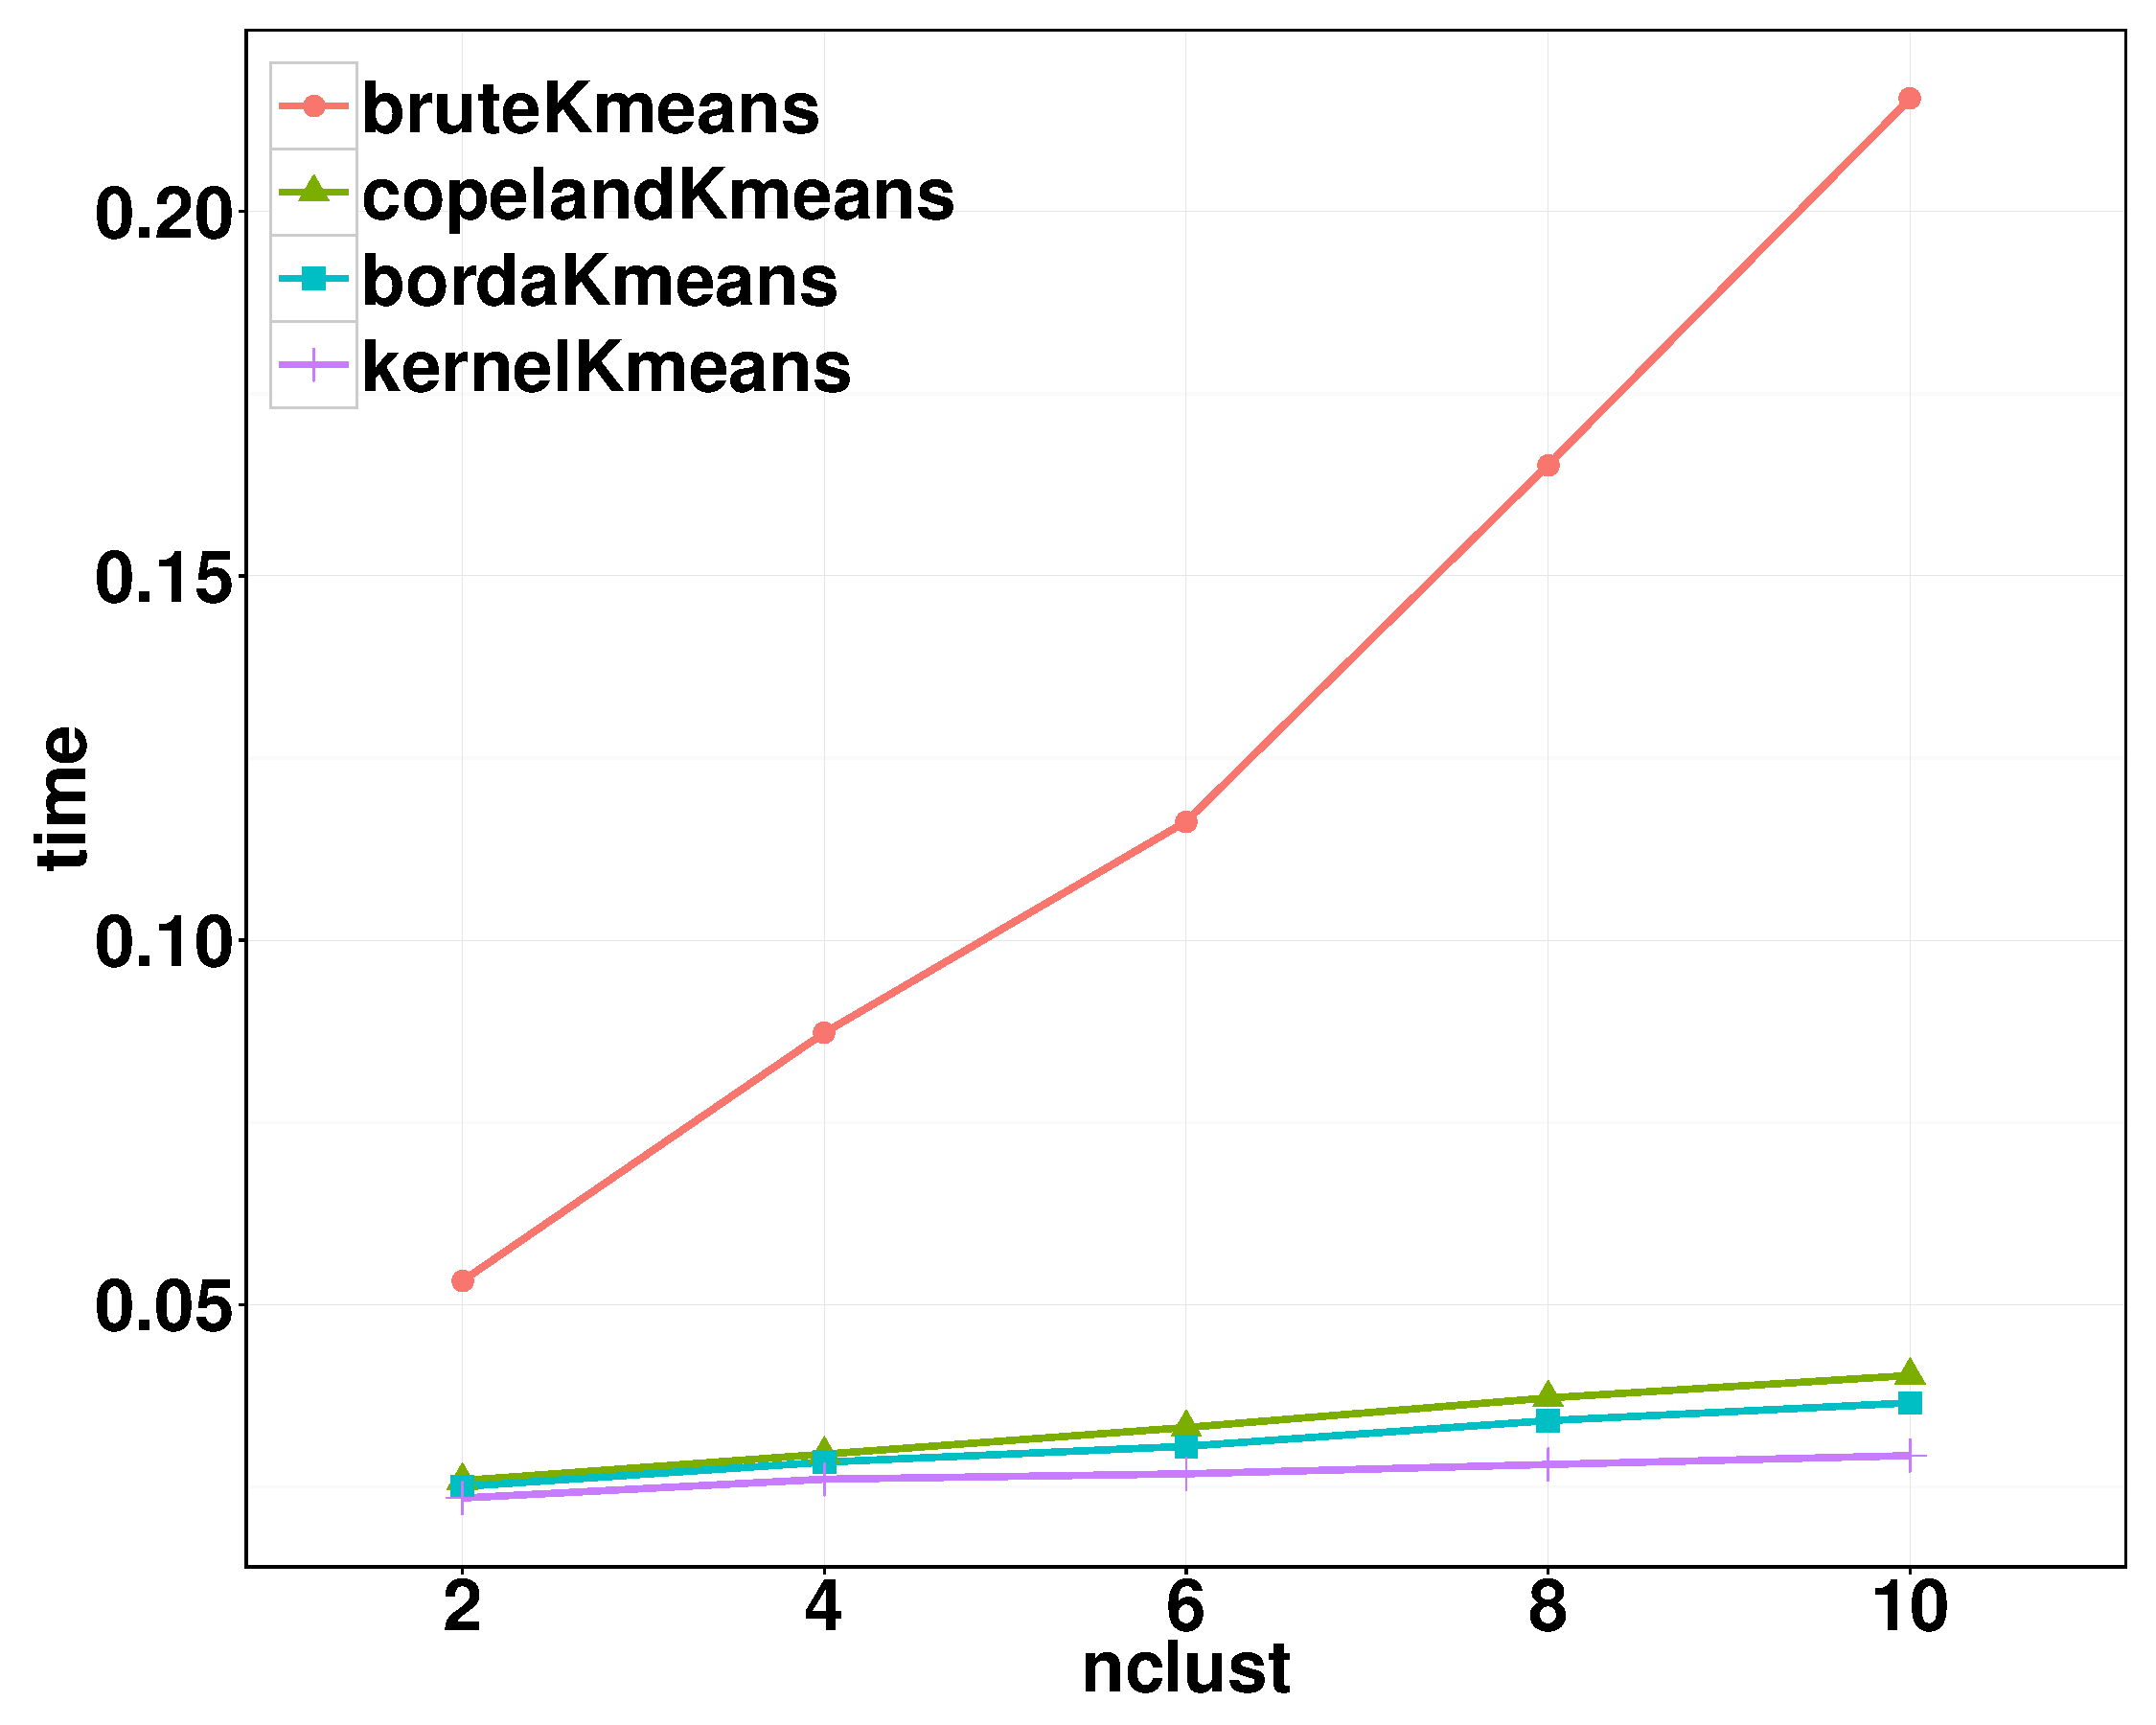
\includegraphics[width=\columnwidth]{ch-kendall/cluster_results/kmeans-time}}
%			\only<5>{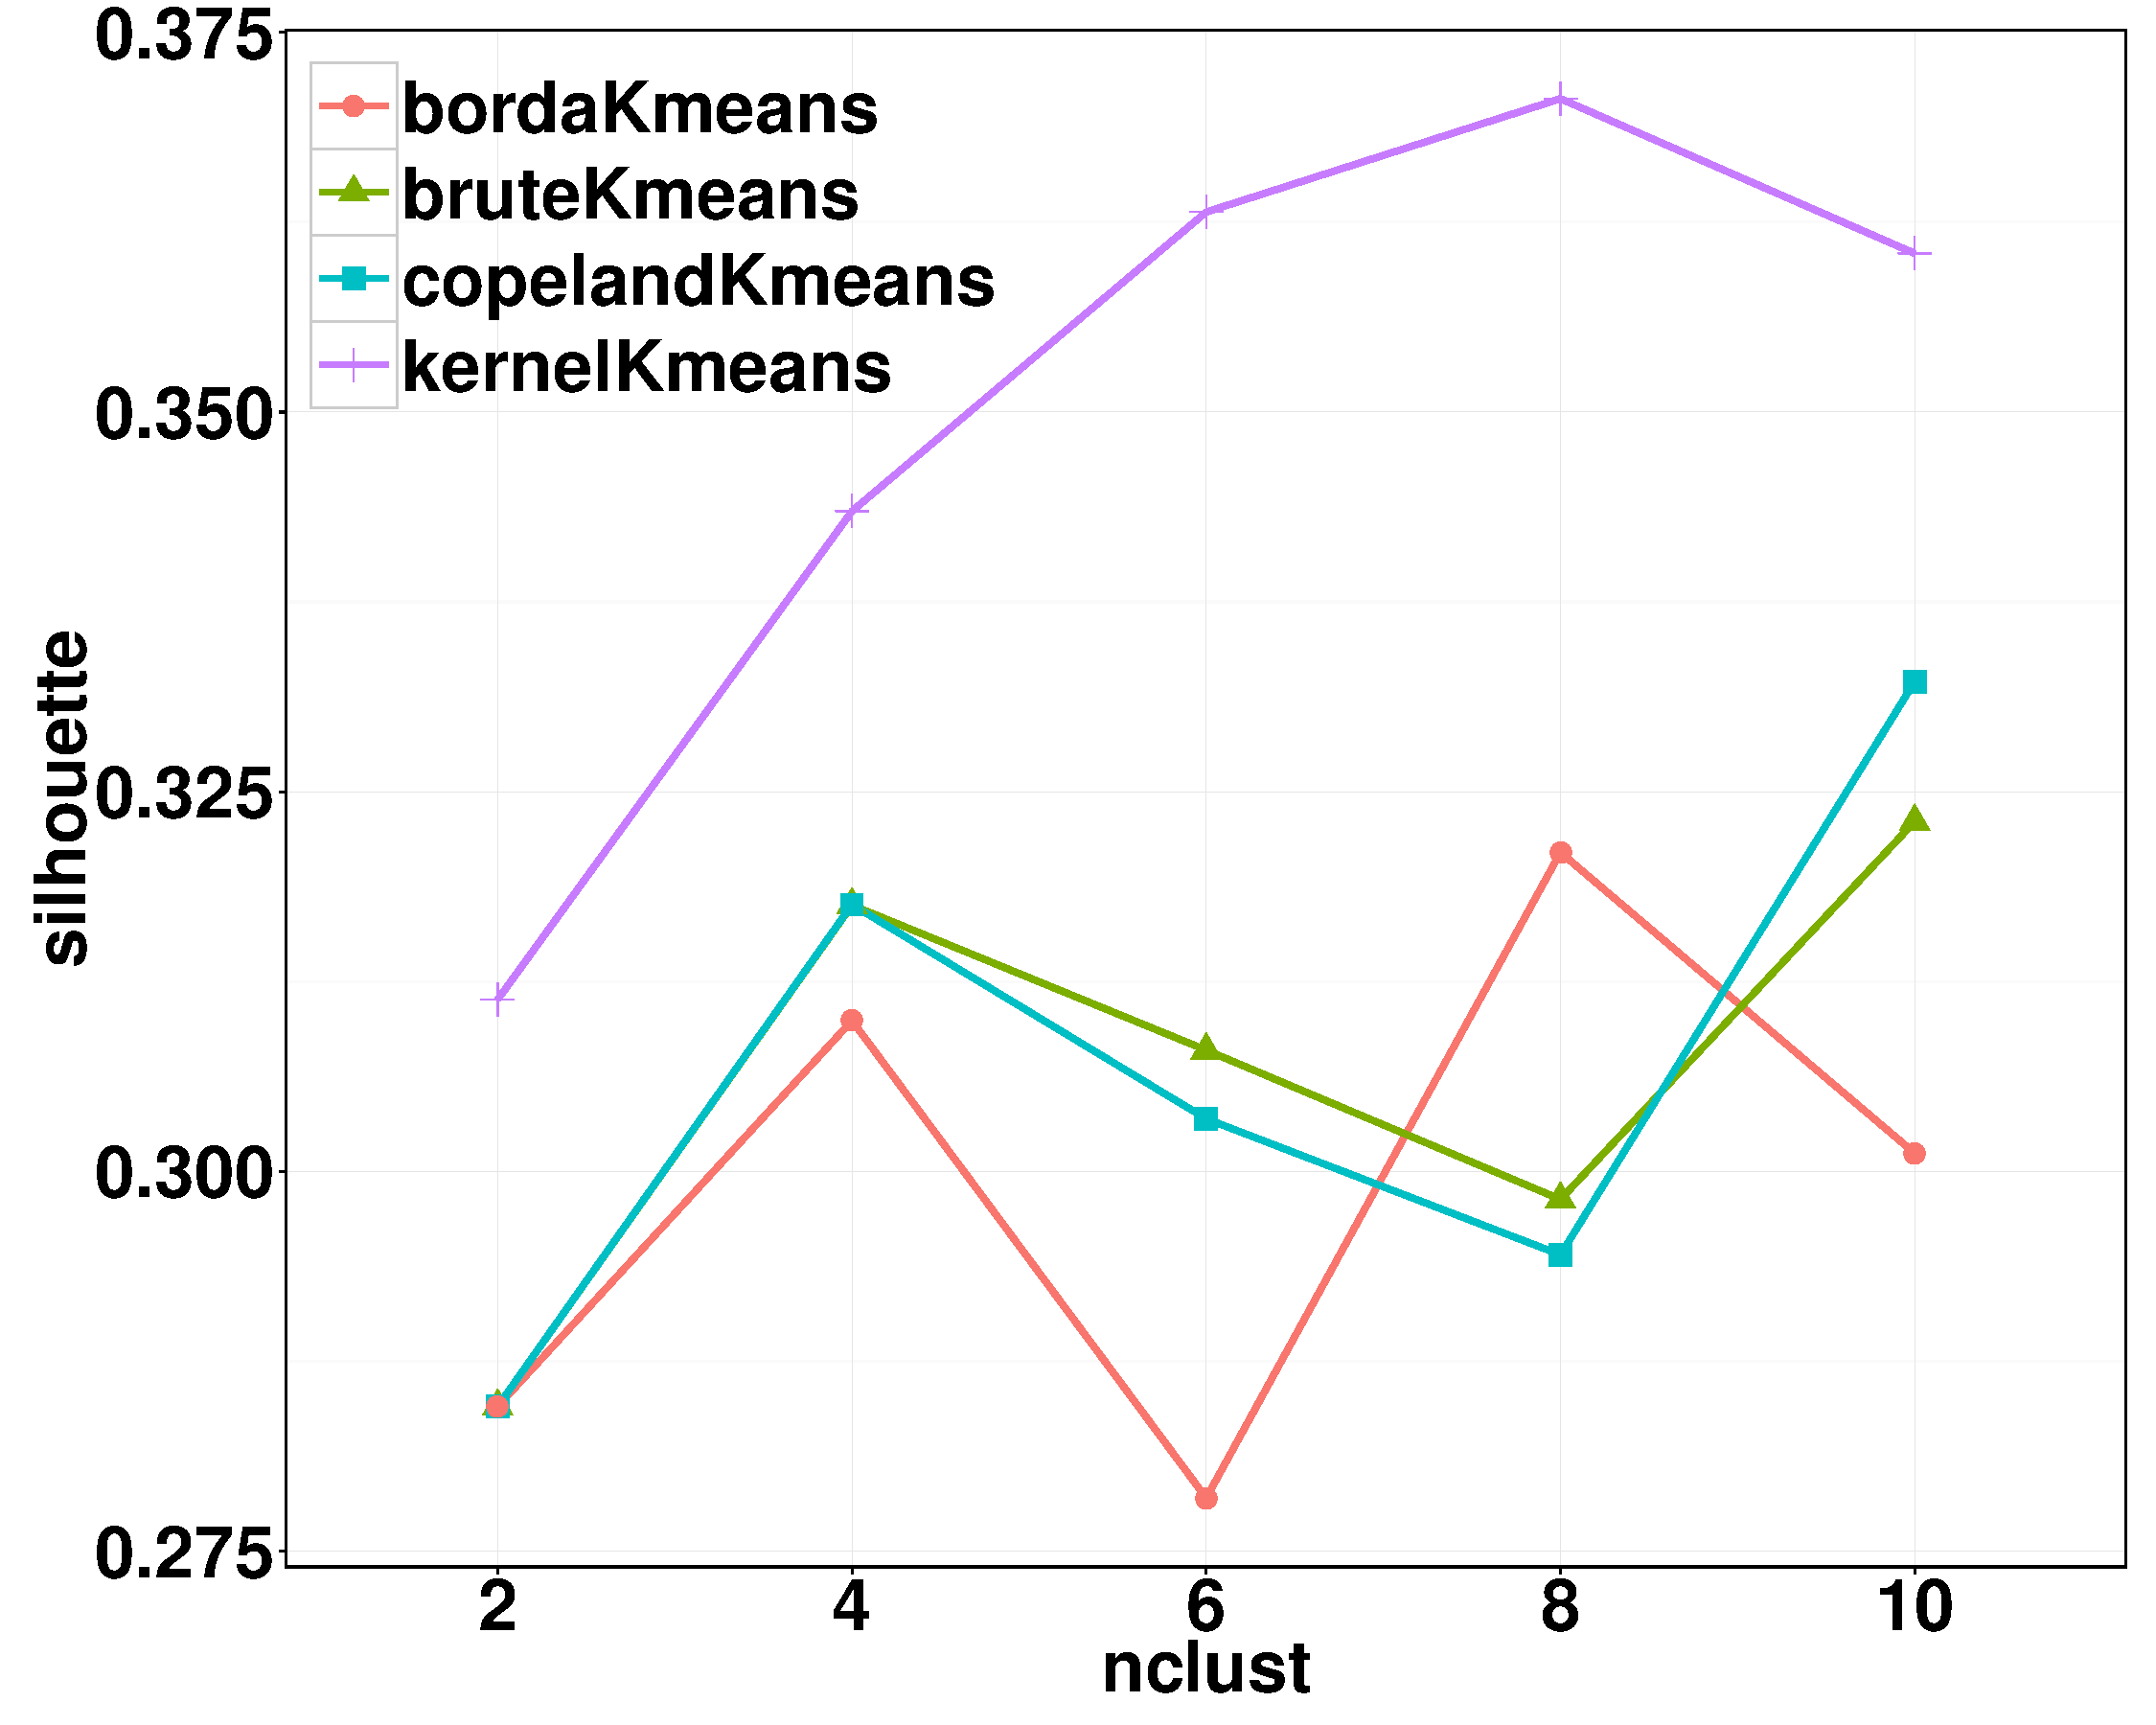
\includegraphics[width=\columnwidth]{ch-kendall/cluster_results/kmeans-silhouette}}
%			\only<6>{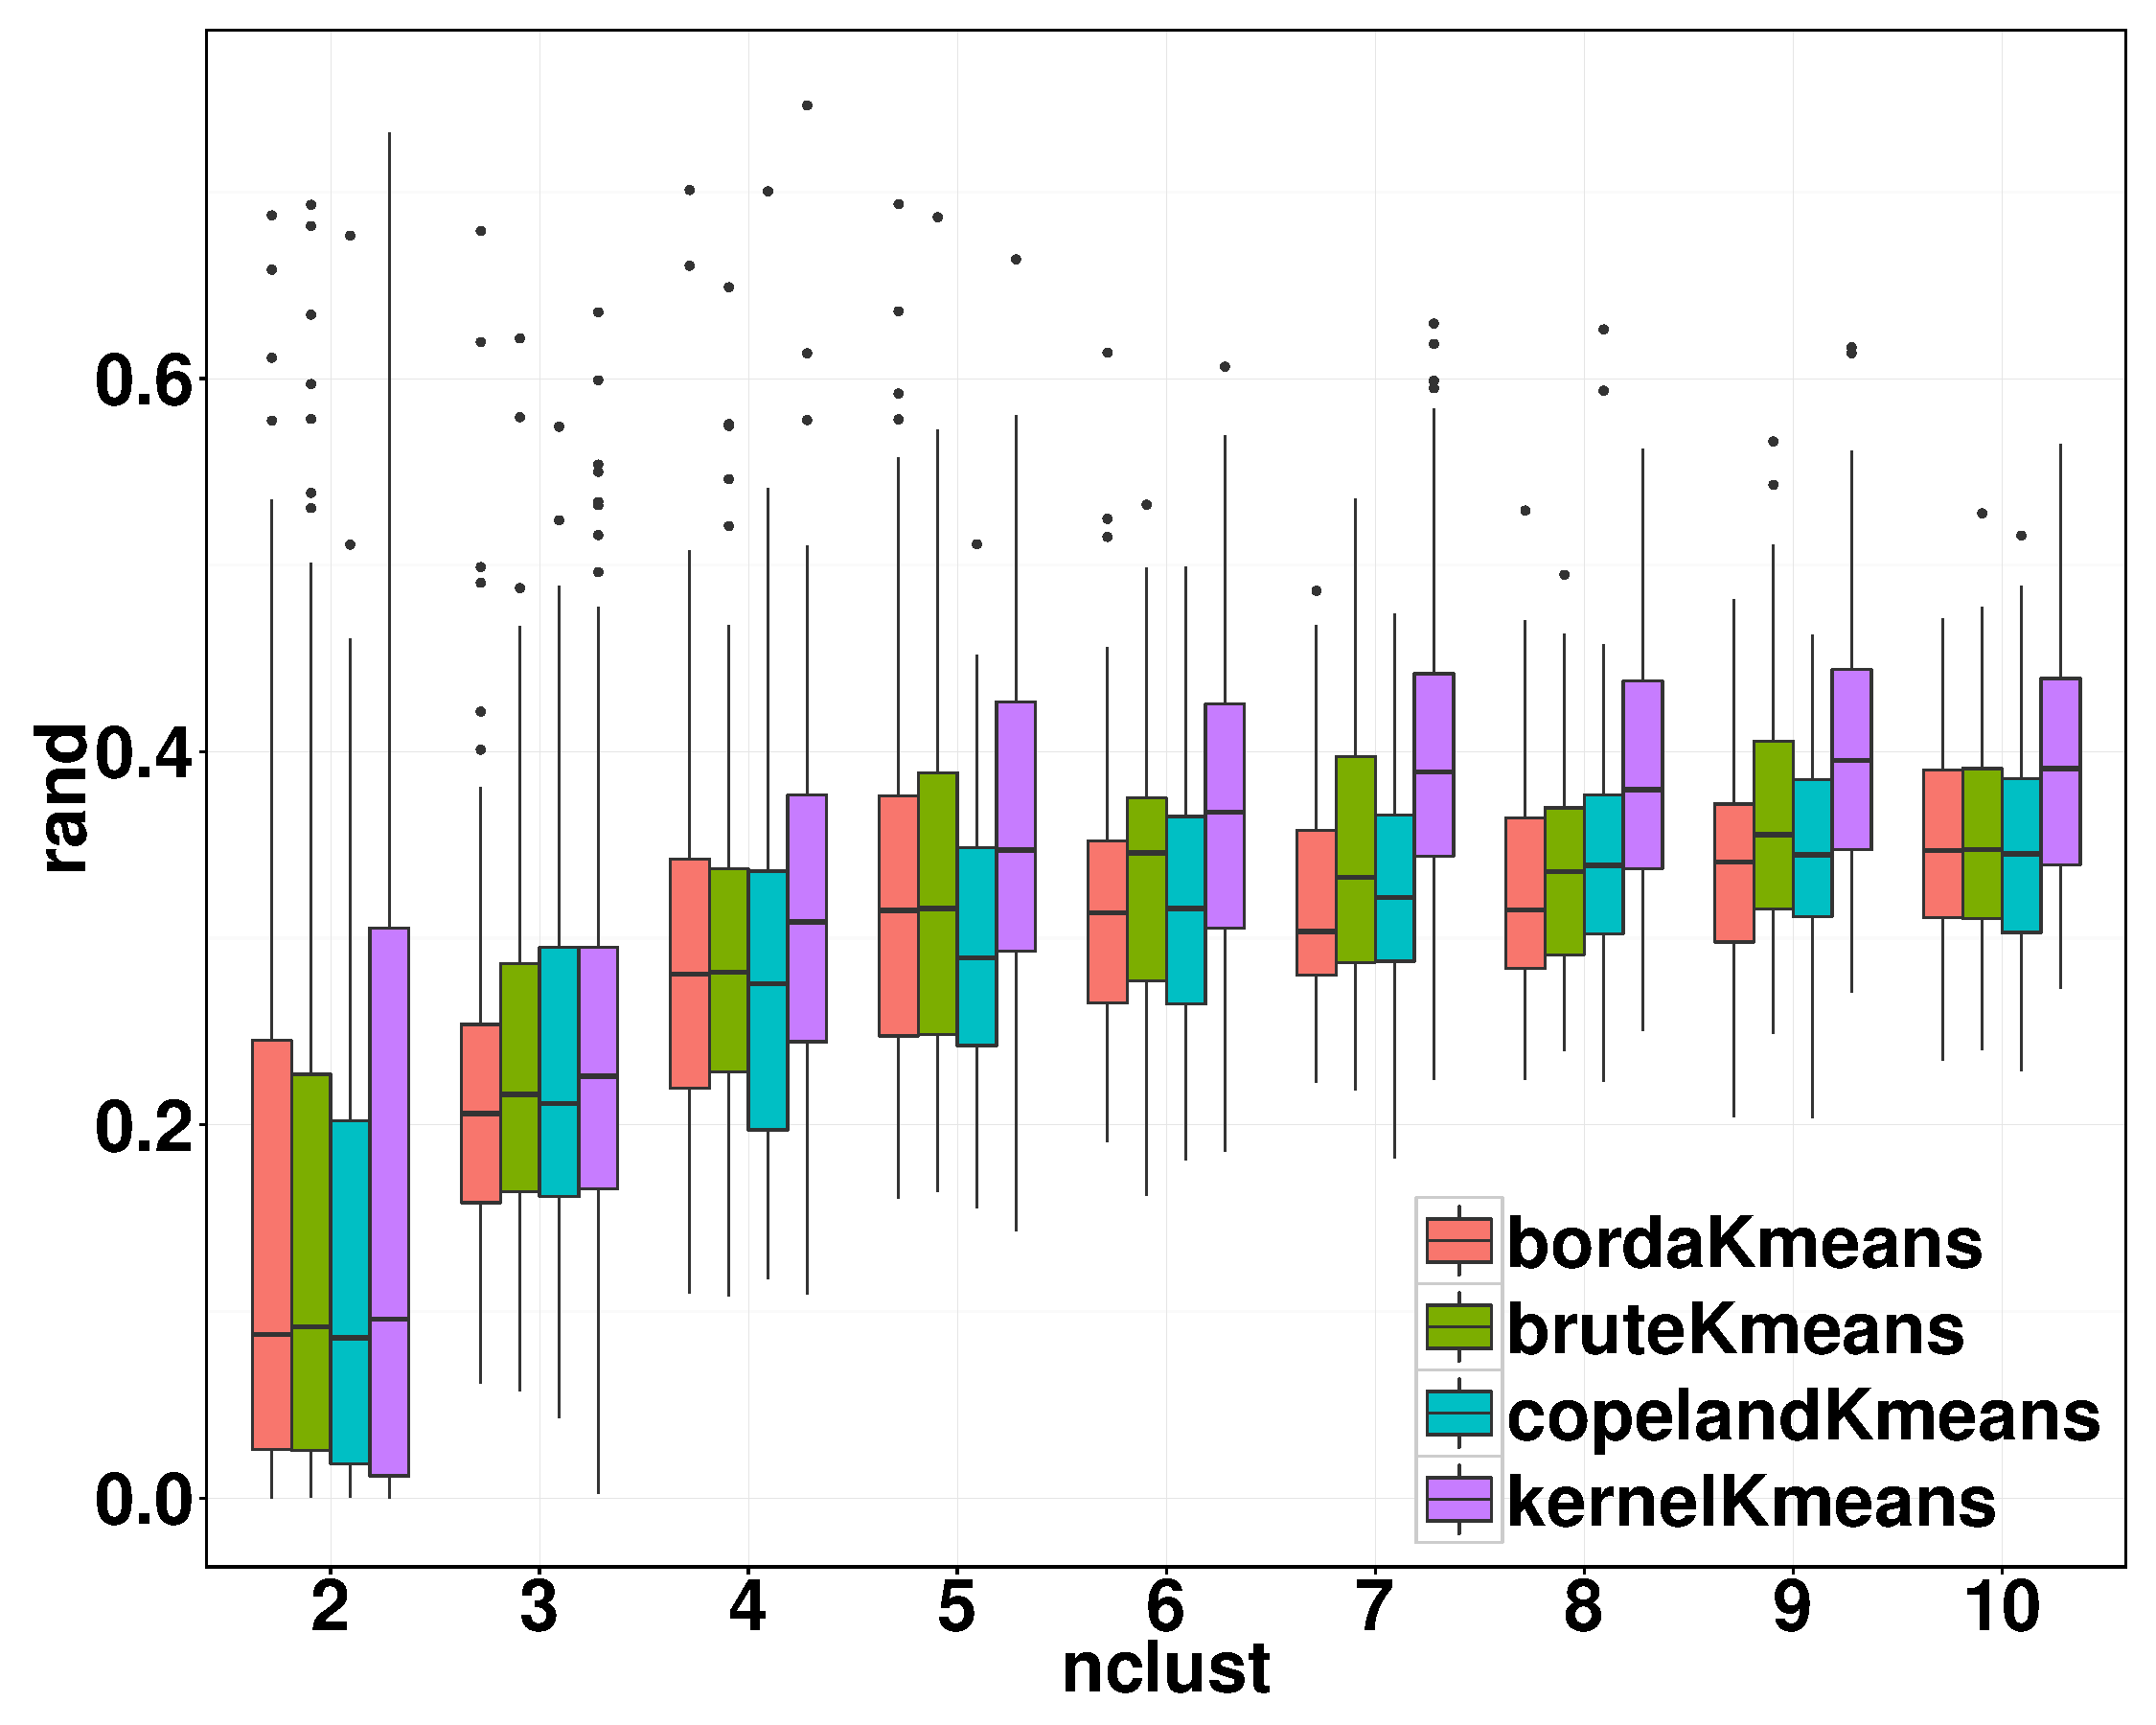
\includegraphics[width=\columnwidth]{ch-kendall/cluster_results/kmeans-stability}}
%		\end{figure} 
%	\>
%	\<{0.5\linewidth}
%		Kendall kernel $k$-means has
%		\begin{itemize}
%			\item<4-6> \alert<4>{Less running time!}
%			\item<5-6> \alert<5>{Higher cluster consistency!}
%			\item<6> \alert<6>{Higher cluster stability!}
%		\end{itemize}
%	\>
%	\)
%	}
	
\end{frame}



\subsection{\scshape Extension (1/2): Partial rankings}
\begin{frame}{\insertsubsection}
	
	\begin{itemize}
		\item An interleaving partial ranking of size $k$ is
		$$ x_{i_1} \succ x_{i_2} \succ \cdots \succ x_{i_k} \,, \quad k\leq n \,, $$
		and a top-$k$ partial ranking is
		$$ x_{i_1} \succ x_{i_2} \succ \cdots \succ x_{i_k} \succ X_{\textrm{rest}} \,, \quad k\leq n \,. $$
		\item A partial ranking is \alert<1>{uniquely represented} by a set of permutations compatible with the observed partial orders.
	\end{itemize}
	
	\pause
	
	\begin{thm}
		For these two particular types of partial rankings, the \alert{convolution kernel} \cite{Haussler1999Convolution} induced by Kendall kernel
	$$ K_\tau^\star (R,R')=\frac{1}{|R||R'|} \sum_{\sigma\in R} \sum_{\sigma'\in R'}K_\tau (\sigma, \sigma') $$
	can be evaluated in \alert{$O(k\log k)$} time.
	\end{thm}
	
\end{frame}


\subsection{\scshape Extension (2/2): Uncertain rankings}
\begin{frame}{\insertsubsection}
	
	\only<1-2>{
	\([c]
	\<{0.55\linewidth}
	\begin{itemize}
		\item Recall for real-valued vectors, Kendall embedding is \alert{binary}\only<2->{ thus sensitive to ``almost ties''},
		$$ \phi(\xb) = \left( \sgn(x_i-x_j) \right)_{1\leq i < j \leq n} \,. $$
		\item Kendall kernel is defined by
		$$
		K_\tau(\xb,\xb') = \phi(\xb)^\top \phi(\xb') \,.
		$$
	\end{itemize}
	\vskip -0.7cm
	\begin{figure}
	\centering
		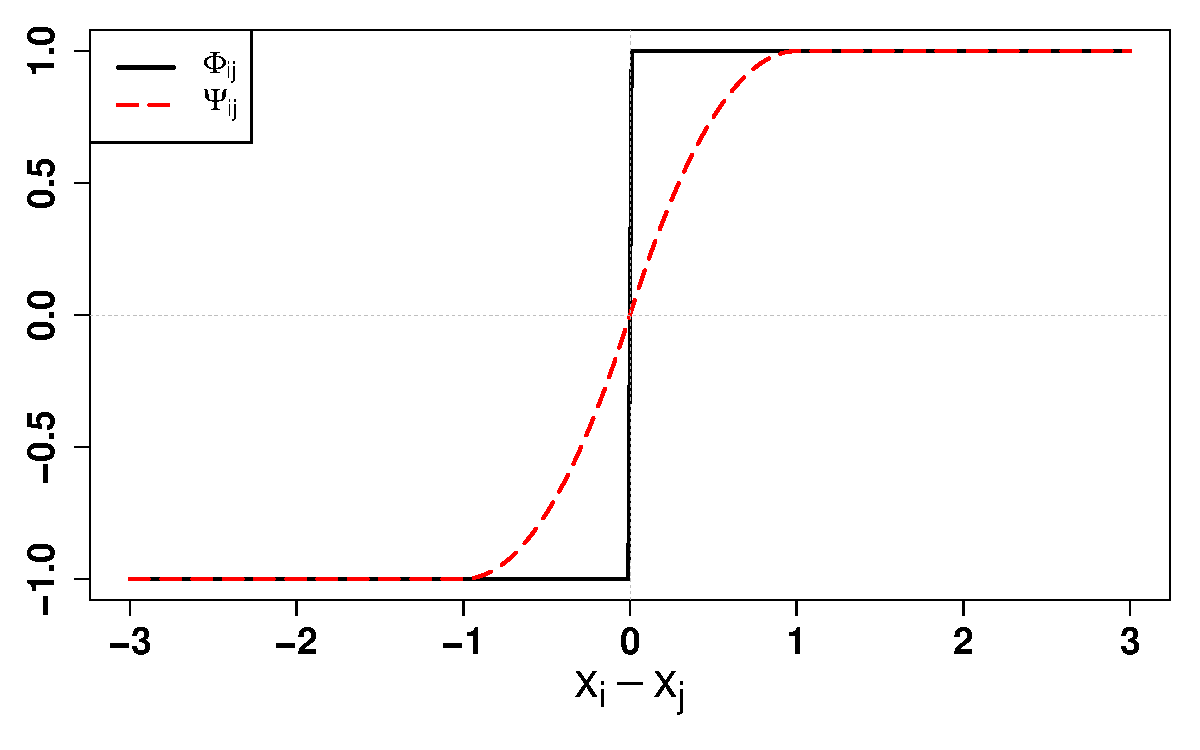
\includegraphics[width=0.8\columnwidth]{ch-kendall/figures/smoothheaviside}
	\end{figure}
	\>
	\<{0.55\linewidth}
		\uncover<2>{
		\vskip -1.5cm
		\begin{itemize}
			\item<2-> Now consider a \alert{continuous} embedding by
			$$
			\psi(\xb) = \EE \phi(\xb + \epsilon) \,,
			$$
			where $\epsilon \sim \br{\mathcal{U}\sqb{-\frac{a}{2}, \frac{a}{2}}}^n \,.$
			\item<2-> Corresponding kernel is defined by
			\begin{equation*}
			\begin{split}
				G(\xb,\xb') & = \psi(\xb)^\top \psi(\xb') \\
				& = \EE K_\tau (\xb + \epsilon, \xb' + \epsilon') \,.
			\end{split}
			\end{equation*}
		\end{itemize}
		}
	\>
	\)
	}
	
	\only<3-5>{
		\begin{itemize}
			\item The \alert<3>{distributional kernel} \cite{Muandet2012Learning} induced by Kendall kernel is defined by
			$$
			G(\xb,\xb') = \psi(\xb)^\top \psi(\xb')
			\only<4->{= \EE K_\tau (\xb + \epsilon, \xb' + \epsilon')}
			\,. $$
			\vskip -0.1cm
			\begin{itemize}
				\item[-] Can be exactly computed in \alert<3>{$O(n^2)$} time.
				\item[-]<4-> Can be approximately computed in \alert<4>{$O(D^2 n \log n)$} time by Monte-Carlo approximation:
				$$ G_D \br{\xb,\xb'} = \frac{1}{D^2} \sum_{i,j=1}^D K_\tau (\xb+\epsilon^{(i)}, \xb' + \epsilon'^{(j)}) \,. $$
			\end{itemize}
		\end{itemize}
	}
	
	\only<5>{
	\begin{thm}
		Training a standard SVM with $m$ samples and $n$ features, using $G_D$ is faster than $G$ for the same statistical accuracy when $m = o(n^{1/3})$.
	\end{thm}
	}
	
	\only<6->{
	\([c]
	\<{0.65\linewidth}
		\begin{figure}
			\only<6>{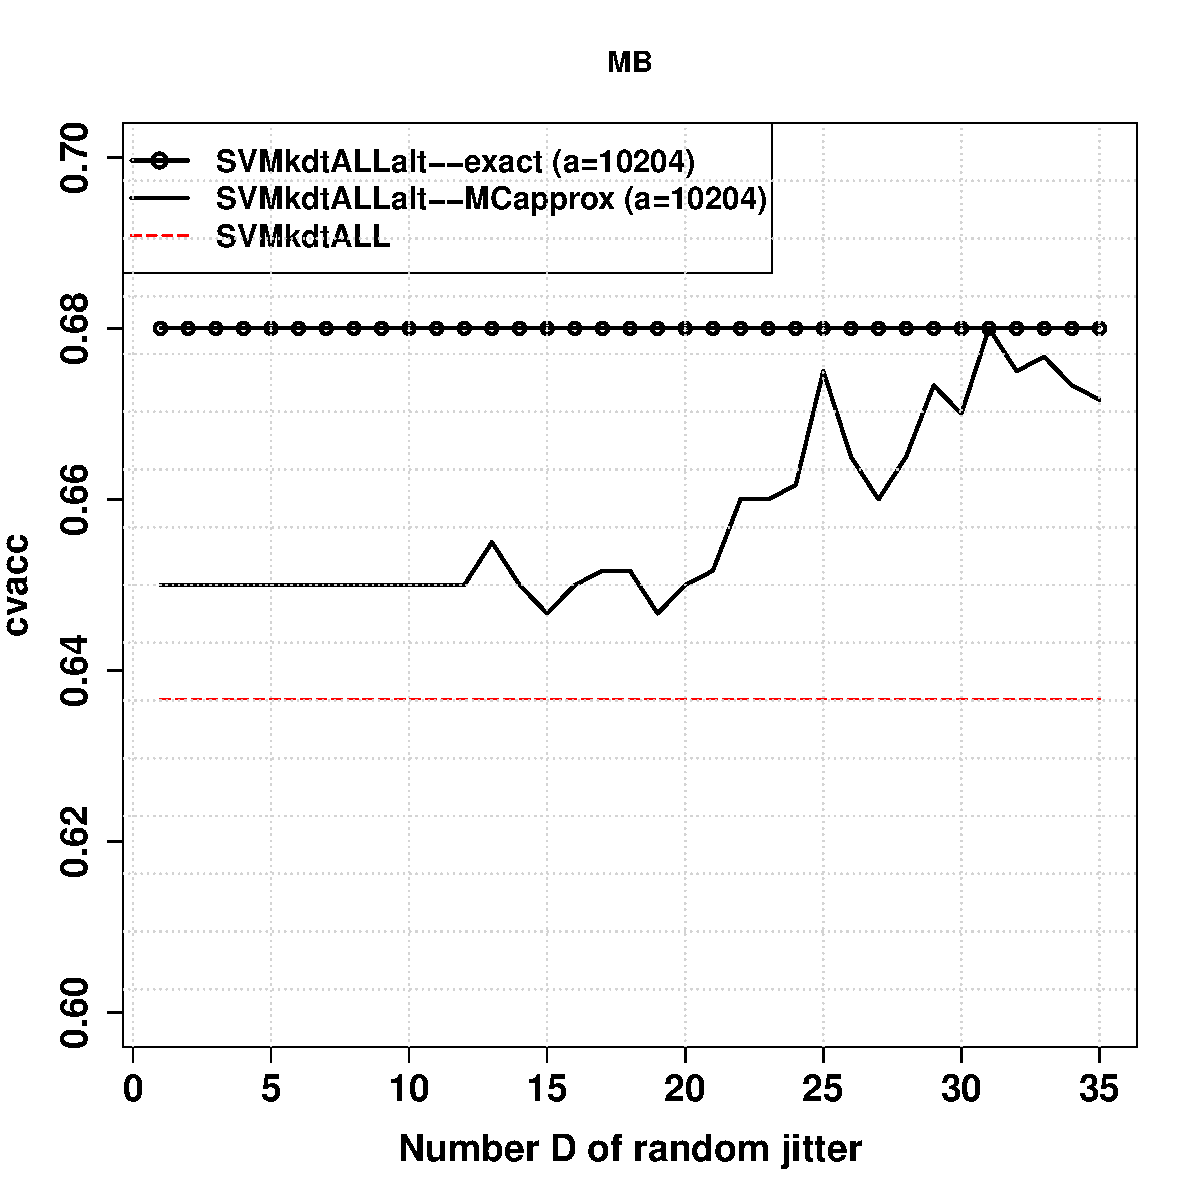
\includegraphics[width=\columnwidth]{ch-kendall/clasf_results/acc_approxSingleWindow}}
		\end{figure}
	\>
	\<{0.5\linewidth}
		Kendall kernel Flex-SVM \cite{Muandet2012Learning} has
		\begin{itemize}
			\item<6> \alert<6>{Improved accuracy!}
		\end{itemize}
	\>
	\)
	}
	
\end{frame}


\subsection{\scshape Mallows kernel for permutations}
\begin{frame}{\insertsubsection}
	
	\([b]
	\<{0.75\linewidth}
	\begin{itemize}
		\item The Mallows kernel for permutations is defined for any $\lambda \geq 0$ by
		$$
			K_M^\lambda (\sigma, \sigma') := e^{-\lambda d(\sigma, \sigma')} \,.
		$$
		\item<2-> Relation to diffusion kernel on $\Sn$:
	\end{itemize}
	\>
	\hspace{-1cm}
	\<{0.4\linewidth}
		\begin{figure}
			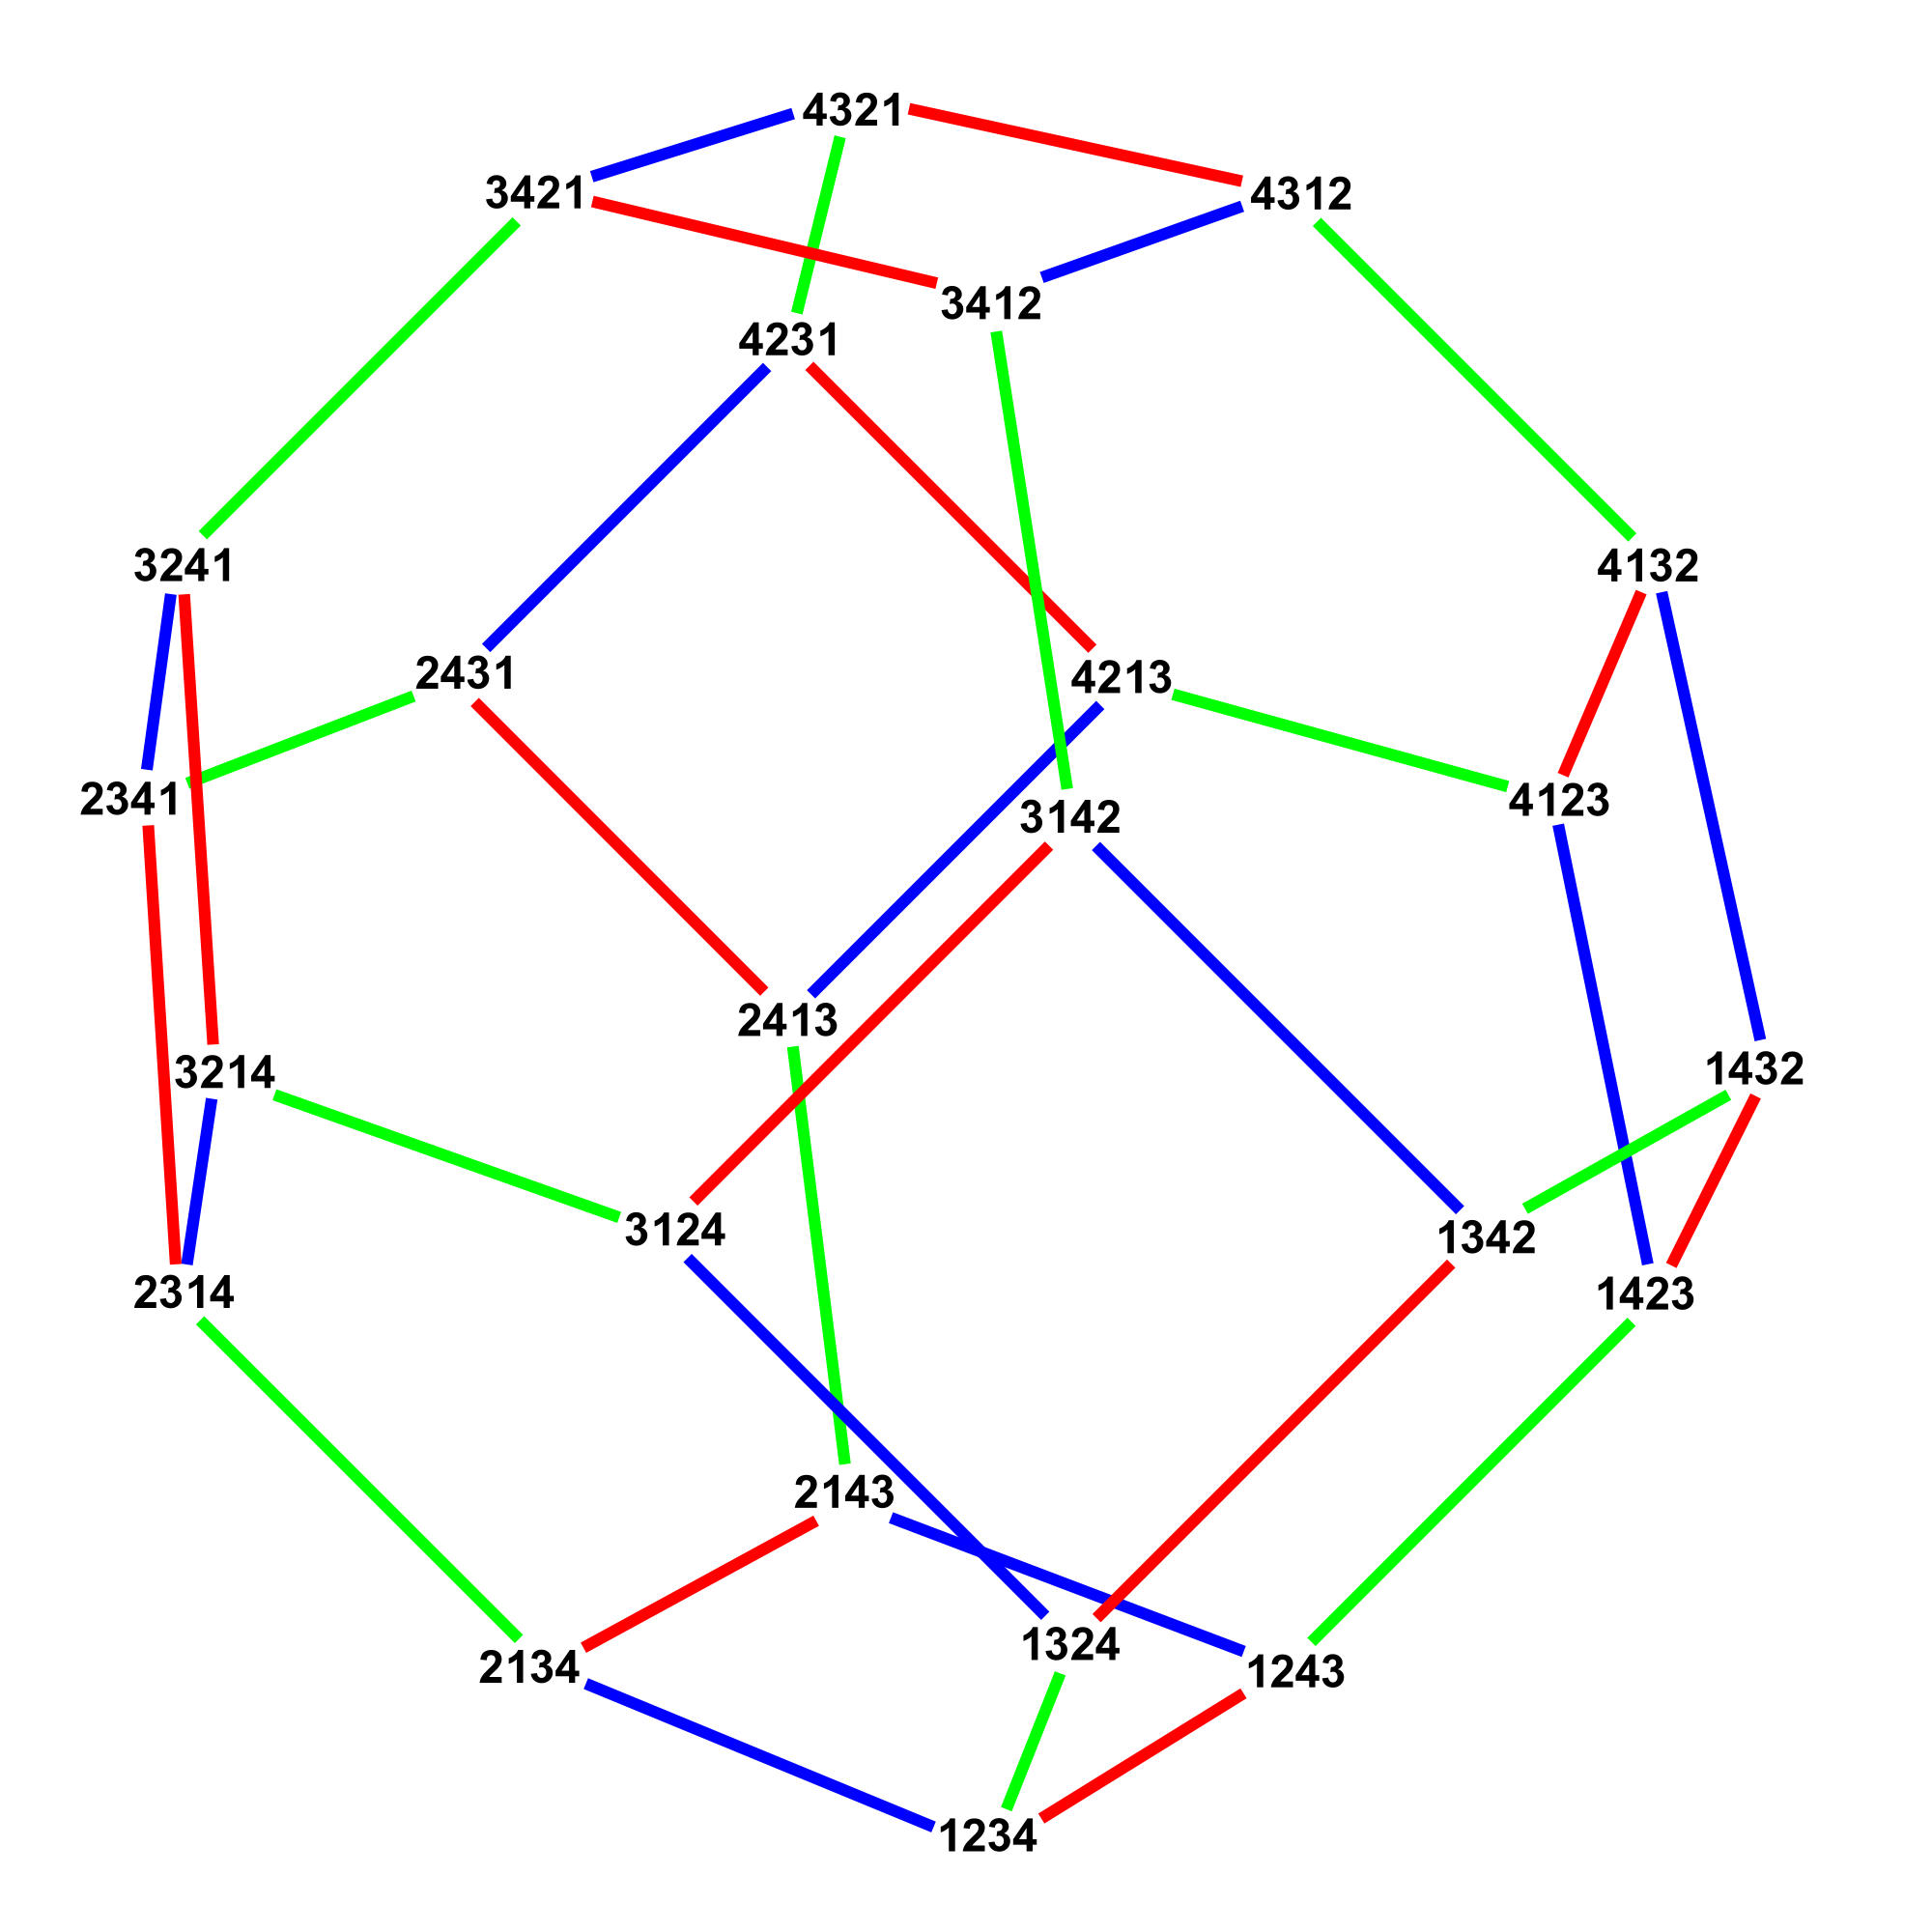
\includegraphics[width=0.7\columnwidth]{ch-kendall/figures/permutahedron}
			\vspace{-0.5cm}
			\caption{Cayley graph of $\mathbb{S}_4$.}
		\end{figure}
	\>
	\)
	
	\only<2->{
	\vskip -0.3cm
	\begin{table}
	\centering
	\footnotesize
	\renewcommand{\arraystretch}{1.5}
	\begin{tabular}{c|cc}
		\hline
		Kernel & Diffusion kernel & Mallows kernel \\\hline
		Definition & $\sqb{e^{-\lambda \Delta}}_{\sigma,\sigma'}$ & $e^{-\lambda d(\sigma, \sigma')}$ \\
		Positive definiteness & $\checkmark$ & $\checkmark$ \\
		Graph interpretation & Diffusion process & Shortest path \\
		Time complexity & $O(n^n)$ & $O(n \log n)$ \\
		Reference & \cite{Kondor2002Diffusion} & \cite{Jiao2015Kendall} \\
		\hline
	\end{tabular}
	\end{table}
	}
	
\end{frame}


\subsection{\scshape Conclusion and future directions}
\begin{frame}{\insertsubsection}
	
	\begin{itemize}
		\item We have shown
		\begin{itemize}
		 \item[-] Kendall and Mallows kernels are computationally attractive, positive definite kernels on $\Sn$.
		 \item[-] Kendall distance for permutations is negative definite.
		 \item[-] Applications involving biomedical classification, clustering and rank aggregation in social choice theory.
		 \item[-] Extensions to partial rankings and uncertain rankings.
		\end{itemize}
		
		\pause
		
		\item We are currently working on extending Kendall kernel to
		\begin{itemize}
			\item[?] Weighted pairwise comparison.
			\item[?] higher-order (such as three-way) comparison.
			\item[?] partially ordered set.
		\end{itemize}
	\end{itemize}
	
\end{frame}

\section{\scshape Learning on graphs}


\begin{frame}
	
	\addsectiontitlepage
	
	\(
	\<{0.4\linewidth}
	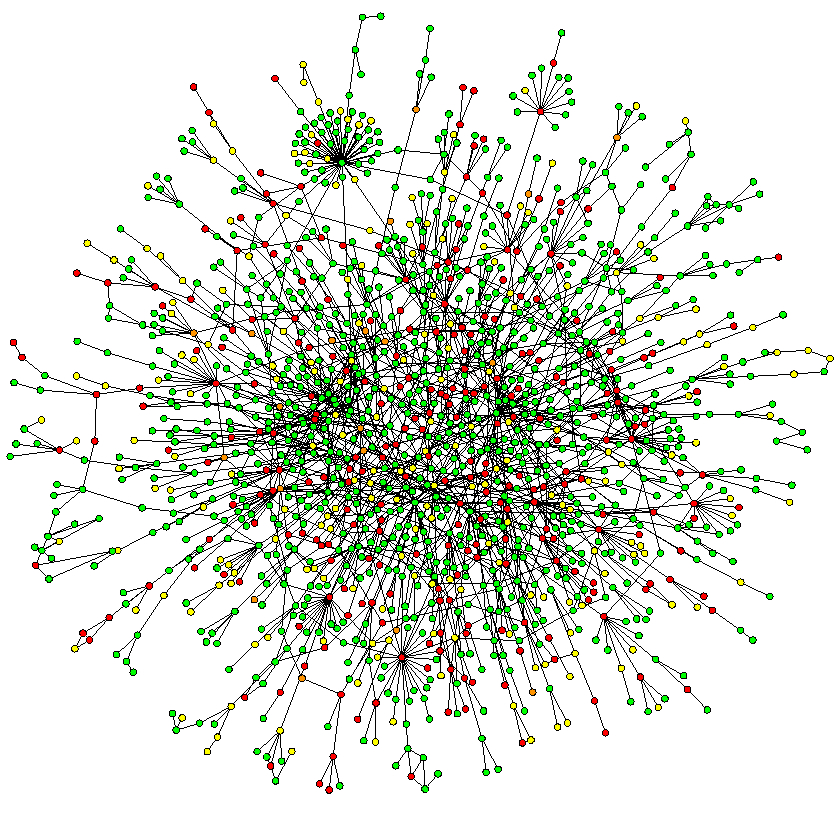
\includegraphics[width=\columnwidth]{slides/ppi}
	\>
	
	\<{0.55\linewidth}
	\begin{footnotesize}
	\textbf{Working Papers and Preprints}
	\begin{itemize}
		\item \nocite{Jiao2017Network} Jiao, Y., Vert, J.-P. Technical report.
		\item \nocite{Jiao2017Signaling} Jiao, Y., Hidalgo, M. R., \c{C}ubuk, C., Amadoz, A., Carbonell-Caballero, J., Vert, J.-P., Dopazo, J. Preprint bioRxiv-132357. (*)
	\end{itemize}
	\end{footnotesize}
	\>
	\)
	
\end{frame}


\subsection{\scshape Motivation recap}
\begin{frame}{\insertsubsection}
	
	\begin{itemize}
		\item Data: 
		\begin{figure}
			\centering
			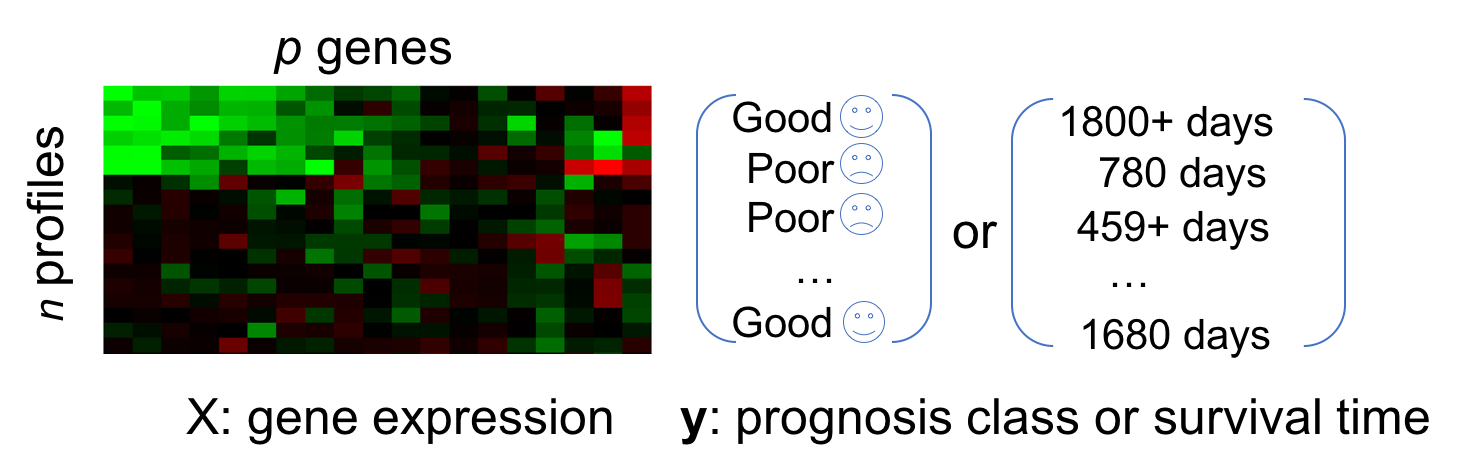
\includegraphics[width=0.7\linewidth]{slides/prognosis}%
			\hskip 0.1cm%
			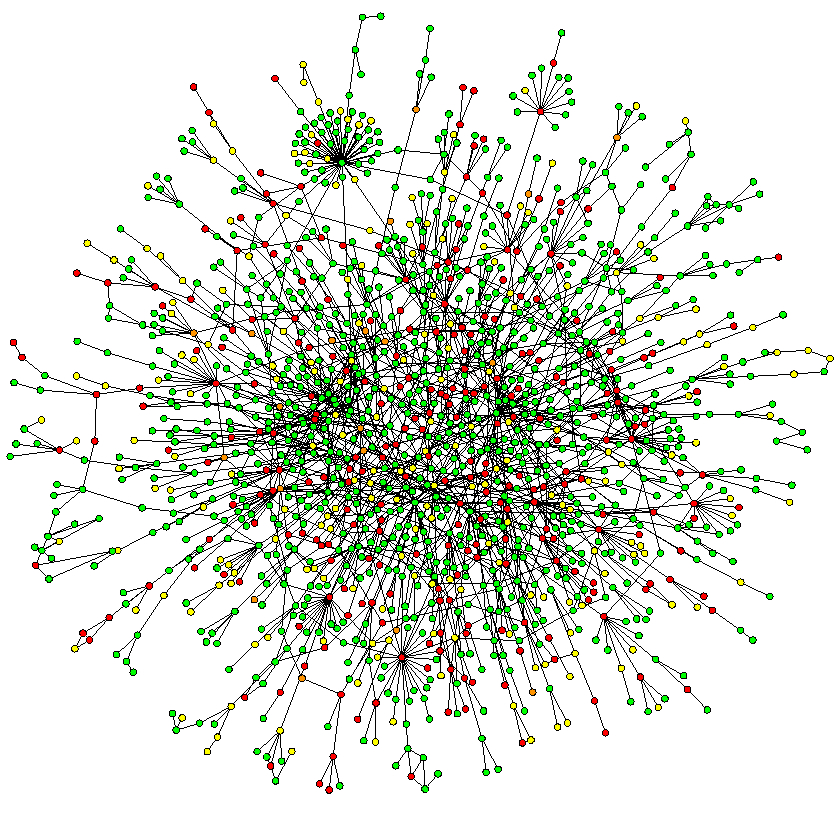
\includegraphics[width=0.25\linewidth]{slides/ppi}
		\end{figure}
		
		\item Goal: Learn to predict $y$ from a patient's profile $\mathbf{x}$.
		\begin{itemize}
			\item[-] Network-guided analysis.
			\item[-] Classification or survival analysis with linear models.
			\item[-] Structured gene/subnetwork selection by regularization.
		\end{itemize}
	\end{itemize}
	
\end{frame}


\section{\scshape Conclusion}


\begin{frame}{\insertsection}
	
\end{frame}


\begin{frame}{Acknowledgments}
	
\end{frame}


\begin{frame}[allowframebreaks]{References}
	
	\tiny
	\bibliography{mybib}
	\bibliographystyle{apalike}
	
\end{frame}



\end{document}
